% generated from JIRA project LVV
% using template at /usr/local/lib/python3.7/site-packages/docsteady/templates/se-tpr.latex.jinja2.
% using docsteady version 1.2rc21
% Please do not edit -- update information in Jira instead

\documentclass[SE,lsstdraft,STR,toc]{lsstdoc}
\usepackage{geometry}
\usepackage{longtable,booktabs}
\usepackage{enumitem}
\usepackage{arydshln}
\usepackage{attachfile}
\usepackage{array}

\newcolumntype{L}[1]{>{\raggedright\let\newline\\\arraybackslash\hspace{0pt}}p{#1}}

\input meta.tex

\newcommand{\attachmentsUrl}{https://github.com/\gitorg/\lsstDocType-\lsstDocNum/blob/\gitref/attachments}
\providecommand{\tightlist}{
  \setlength{\itemsep}{0pt}\setlength{\parskip}{0pt}}

\setcounter{tocdepth}{4}

\begin{document}

\def\milestoneName{Camera Hexapod Functional Re-verification}
\def\milestoneId{LVV-P63}
\def\product{SIT-COM Integration}

\setDocCompact{true}

\title{LVV-P63: Camera Hexapod Functional Re-verification Test Plan and Report}
\setDocRef{\lsstDocType-\lsstDocNum}
\date{\vcsdate}
\author{ Austin Roberts }

% Most recent last
\setDocChangeRecord{
\addtohist{}{2019-12-06}{First Draft}{Austin Roberts}
}

\setDocCurator{Austin Roberts}
\setDocUpstreamLocation{\url{https://github.com/lsst-dm/\lsstDocType-\lsstDocNum}}
\setDocUpstreamVersion{\vcsrevision}



\setDocAbstract{
This is the test plan and report for LVV-P63 (Camera Hexapod Functional Re-verification),
an LSST milestone pertaining to the System Engineering Subsystem.
}


\maketitle

\section{Introduction}
\label{sect:intro}


\subsection{Objectives}
\label{sect:objectives}

 The objective of this test plan is to re-verify the functional
requirements of the Camera Hexapod's hardware and software, after
shipment from the vendors facility to the Summit, as defined in \citeds{LTS-206}
and \citeds{LTS-160}. This test campaign will only exercise the functionality
that was executed previously and meets the following criteria:

\begin{itemize}
\tightlist
\item
  Only requires the vendors EUI software and hardware via local control
\item
  Only requires a laser tracker
\item
  Does \textbf{NOT} require the camera rotator to be loaded with the
  camera simulated mass or actual camera hardware
\item
  Does not require for the CCW or Camera Rotator to be operable.
\end{itemize}

The hardware and software functional requirements were previously
verified during the test campaign by the vendor at the vendors facility
and accepted by LSST during the Factory Acceptance Test review.


\subsection{System Overview}
\label{sect:systemoverview}

 The Camera Hexapod is mounted to the Camera Rotator with the primary
function of aligning the camera with the optical path of the telescope.


\subsection{Document Overview}
\label{sect:docoverview}

This document was generated from Jira, obtaining the relevant information from the
\href{https://jira.lsstcorp.org/secure/Tests.jspa\#/testPlan/LVV-P63}{LVV-P63}
~Jira Test Plan and related Test Cycles (
\href{https://jira.lsstcorp.org/secure/Tests.jspa\#/testCycle/LVV-C114}{LVV-C114}
).


Section \ref{sect:intro} provides an overview of the test campaign, the system under test (\product{}),
the applicable documentation, and explains how this document is organized.
Section \ref{sect:testplan} provides additional information about the test plan, like for example the configuration
used for this test or related documentation.
Section \ref{sect:personnel} describes the necessary roles and lists the individuals assigned to them.

Section \ref{sect:overview} provides a summary of the test results, including an overview in Table \ref{table:summary},
an overall assessment statement and suggestions for possible improvements.
Section \ref{sect:detailedtestresults} provides detailed results for each step in each test case.

The current status of test plan \href{https://jira.lsstcorp.org/secure/Tests.jspa\#/testPlan/LVV-P63}{LVV-P63} in Jira is \textbf{ Approved }.

\subsection{References}
\label{sect:references}
\renewcommand{\refname}{}
\bibliography{lsst,refs,books,refs_ads,local}


\newpage
\section{Test Plan Details}
\label{sect:testplan}


\subsection{Data Collection}

  Observing is not required for this test campaign.

\subsection{Verification Environment}
\label{sect:hwconf}
  The Camera Hexapod will be verified in a climate controlled environment
on the 3rd floor of the Summit Facility integrated with the Camera Cable
Wrap on the Camera Cart.

  \subsection{Entry Criteria}
  In order to test the Camera Hexapod functionality, the following
criteria must be met first:

\begin{itemize}
\tightlist
\item
  All the test setup for the Data Acquisition system must be completed
  and ready to record data for the laser tracker and current probes
\item
  The Laser tracker and SMR's are installed and setup
\item
  The Inductive current probes are installed and setup
\item
  All utilities and electrical connections are hooked up and allow the
  Camera Hexapod to be powered on and controlled
\item
  The EFD must be set up to be able to store events and telemetry data
\end{itemize}

  \subsection{Exit Criteria}
  In order for this event to be considered complete, the following
criteria must be met:

\begin{itemize}
\tightlist
\item
  Raw test data, events, and telemetry have been saved for the Camera
  Hexapod.
\item
  All test data has been analyzed and post processed.
\item
  All test steps have been statused in the Jira Test Cases within this
  Test Plan and actual results populated as required.
\item
  A summary of the results of the test campaign has been captured in the
  Overall Assessment and Recommended Improvements fields of this Test
  Plan
\item
  A link to the verification artifacts used to produce the summary of
  results has been populated in the Verification Artifacts field of this
  Test Plan
\item
  Any failures have been captured in the
  \href{https://jira.lsstcorp.org/projects/FRACAS/issues/}{FRACAS}
  project
\end{itemize}


\subsection{Related Documentation}

The documentation related to this test campaign should be provided in the following DocuShare Collection
(as per Verification Artifacts in Jira test plan LVV-P63).

\begin{itemize}
\item DocuShare Collection Not Specified
\end{itemize}

\begin{longtable}{rp{10cm}l}
\multicolumn{3}{c}{Jira Attachments} \\ \hline
LVV-C114 & LSSTHexapods-RotatorAcceptanceTestProcedure\_re-verification\_hardware.v.2.pdf & \attachfile{attachments/LSSTHexapods-RotatorAcceptanceTestProcedure_re-verification_hardware.v.2.pdf}\\ \hline
LVV-C114 & LSSTHexapods-RotatorAcceptanceTest\_re-verif.\_(hardwarereport).v.2.pdf & \attachfile{attachments/LSSTHexapods-RotatorAcceptanceTest_re-verif._(hardwarereport).v.2.pdf}\\ \hline
LVV-C114 & Hex.xyzRxRy.3.3.1.v.2.xlsx & \attachfile{attachments/Hex.xyzRxRy.3.3.1.v.2.xlsx}\\ \hline
      \end{longtable}

All documents provided as attachments in Jira are downloaded to Github and linked here for convenience.
However, since they are not properly versioned, they should be considered informal and therefore
not be part of the verification baseline.


\subsection{PMCS Activity}

Primavera milestones related to the test campaign.

See Epics in Traceability Tab


\newpage
\section{Personnel}
\label{sect:personnel}

The personnel involved in the test campaign is shown in the following table.

{\small
\begin{longtable}{p{3cm}p{3cm}p{3cm}p{6cm}}
\hline
\multicolumn{2}{r}{T. Plan \href{https://jira.lsstcorp.org/secure/Tests.jspa\#/testPlan/LVV-P63}{LVV-P63} owner:} &
\multicolumn{2}{l}{\textbf{ Austin Roberts } }\\\hline
\multicolumn{2}{r}{T. Cycle \href{https://jira.lsstcorp.org/secure/Tests.jspa\#/testCycle/LVV-C114}{LVV-C114} owner:} &
\multicolumn{2}{l}{\textbf{
Undefined }
} \\\hline
\textbf{Test Cases} & \textbf{Assigned to} & \textbf{Executed by} & \textbf{Additional Test Personnel} \\ \hline
\href{https://jira.lsstcorp.org/secure/Tests.jspa#/testCase/LVV-T1598}{LVV-T1598}
& {\small Te-Wei Tsai } & {\small Te-Wei Tsai } &
\begin{minipage}[]{6cm}
\smallskip
{\small  }
\medskip
\end{minipage}
\\ \hline
\href{https://jira.lsstcorp.org/secure/Tests.jspa#/testCase/LVV-T1599}{LVV-T1599}
& {\small Te-Wei Tsai } & {\small Te-Wei Tsai } &
\begin{minipage}[]{6cm}
\smallskip
{\small (1) Software Engineer\\
(1) Hardware Engineer }
\medskip
\end{minipage}
\\ \hline
\href{https://jira.lsstcorp.org/secure/Tests.jspa#/testCase/LVV-T1600}{LVV-T1600}
& {\small Eric Coughlin } & {\small Te-Wei Tsai } &
\begin{minipage}[]{6cm}
\smallskip
{\small (1) Software Engineer\\
(1) Hardware Engineer }
\medskip
\end{minipage}
\\ \hline
\end{longtable}
}

\newpage

\section{Test Campaign Overview}
\label{sect:overview}

\subsection{Summary}
\label{sect:summarytable}

{\small
\begin{longtable}{p{2cm}cp{2.3cm}p{8.6cm}p{2.3cm}}
\toprule
\multicolumn{2}{r}{ T. Plan \href{https://jira.lsstcorp.org/secure/Tests.jspa\#/testPlan/LVV-P63}{LVV-P63}:} &
\multicolumn{2}{p{10.9cm}}{\textbf{ Camera Hexapod Functional Re-verification }} & Approved \\\hline
\multicolumn{2}{r}{ T. Cycle \href{https://jira.lsstcorp.org/secure/Tests.jspa\#/testCycle/LVV-C114}{LVV-C114}:} &
\multicolumn{2}{p{10.9cm}}{\textbf{ Camera Hexapod Re-verification }} & Done \\\hline
\textbf{Test Cases} &  \textbf{Ver.} & \textbf{Status} & \textbf{Comment} & \textbf{Issues} \\\toprule
\href{https://jira.lsstcorp.org/secure/Tests.jspa#/testCase/LVV-T1598}{LVV-T1598}
&  1
& Fail &
\begin{minipage}[]{9cm}
\smallskip

\medskip
\end{minipage}
&
\href{https://jira.lsstcorp.org/browse/FRACAS-28}{FRACAS-28}
\\\hline
\href{https://jira.lsstcorp.org/secure/Tests.jspa#/testCase/LVV-T1599}{LVV-T1599}
&  1
& Initial Pass &
\begin{minipage}[]{9cm}
\smallskip

\medskip
\end{minipage}
&
\\\hline
\href{https://jira.lsstcorp.org/secure/Tests.jspa#/testCase/LVV-T1600}{LVV-T1600}
&  1
& Fail &
\begin{minipage}[]{9cm}
\smallskip

\medskip
\end{minipage}
&
\href{https://jira.lsstcorp.org/browse/DM-23092}{DM-23092}
\href{https://jira.lsstcorp.org/browse/DM-23092}{DM-23092}
\\\hline
\caption{Test Campaign Summary}
\label{table:summary}
\end{longtable}
}

\subsection{Overall Assessment}
\label{sect:overallassessment}

The overall result of this test is: INITIAL PASS.\\[2\baselineskip]

\subsection{Recommended Improvements}
\label{sect:recommendations}

To better test this in the future, the Camera Hexapod should always be
tested starting from the origin to avoid possible hysteresis.
Furthermore, each test step should be repeated at least three times to
ensure the absolute accuracy of the Camera Hexapod.~

\newpage
\section{Detailed Test Results}
\label{sect:detailedtestresults}

\subsection{Test Cycle LVV-C114 }

Open test cycle {\it \href{https://jira.lsstcorp.org/secure/Tests.jspa#/testrun/LVV-C114}{Camera Hexapod Re-verification}} in Jira.

Test Cycle name: Camera Hexapod Re-verification\\
Status: Done

Re-verify the hardware and software requirements for the Camera rotator
that were previously tested by MOOG.

\subsubsection{Software Version/Baseline}
\begin{enumerate}
\tightlist
\item
  Camera Hexapod Control Software with SAL v4.0
\item
  EFD with SAL v4.0
\end{enumerate}

\subsubsection{Configuration}
No varying configuration between test cycles.

\subsubsection{Test Cases in LVV-C114 Test Cycle}

\paragraph{ LVV-T1598 - Camera Hexapod Hardware Functional Re-verification }\mbox{}\\

Version \textbf{1}.
Open  \href{https://jira.lsstcorp.org/secure/Tests.jspa#/testCase/LVV-T1598}{\textit{ LVV-T1598 } }
test case in Jira.

The objective of this test case is to re-verify the functional
requirements of the camera hexapod's hardware, after shipment from the
vendors facility to the Summit, as defined in \citeds{LTS-206}. This test case
will only exercise the functionality that was executed previously and
meets the following criteria:

\begin{itemize}
\tightlist
\item
  Only requires the camera hexapod to be operable
\item
  Only requires the vendors EUI software and hardware via local control
\item
  Only requires a laser tracker
\item
  Does \textbf{NOT} require the camera rotator to be loaded with the
  camera simulated mass or actual camera hardware
\end{itemize}

The hardware functional requirements were previously verified during the
test campaign by the vendor at the vendors facility and accepted by LSST
during the Factory Acceptance Test review. The test procedure used
during the vendor's acceptance testing is the \emph{LSST
Hexapods-Rotator Acceptance Test Procedure} which is attached to this
test case. The test steps of this test case reference that document for
the details on how to perform the test in a similar way as was performed
previously and includes deviations to that document due to the
differences in the verification configuration and deviations to
requirements granted to the vendor by LSST.\\[2\baselineskip]See the
attached \emph{LSST Rotator Hexapod's Manual} for more information on
how to operate the hexapod.

\textbf{ Preconditions}:\\
Prior to the execution of this test case to re-verify the Camera Hexapod
hardware functional requirements, the following Summit tasks must be
completed:

\begin{itemize}
\tightlist
\item
  The Hexapod has been installed on the camera cart

  \begin{itemize}
  \tightlist
  \item
    \url{https://jira.lsstcorp.org/browse/SUMMIT-3224}
  \end{itemize}
\item
  The Hexapod Controller has been deployed on the summit

  \begin{itemize}
  \tightlist
  \item
    \url{https://jira.lsstcorp.org/browse/SUMMIT-3229}
  \end{itemize}
\item
  Boxes for the Hexapod have been transported to the 3rd level

  \begin{itemize}
  \tightlist
  \item
    \url{https://jira.lsstcorp.org/browse/SUMMIT-3230}
  \end{itemize}
\item
  All Hexapod cables and cabinets have been prepared for integration
  with camera cart

  \begin{itemize}
  \tightlist
  \item
    \url{https://jira.lsstcorp.org/browse/SUMMIT-3231}
  \end{itemize}
\item
  The offset has been installed onto the integrating structure

  \begin{itemize}
  \tightlist
  \item
    \url{https://jira.lsstcorp.org/browse/SUMMIT-3293}
  \end{itemize}
\item
  The Camera Hexapod electrical connections have been tested

  \begin{itemize}
  \tightlist
  \item
    \url{https://jira.lsstcorp.org/browse/SUMMIT-3294}
  \end{itemize}
\end{itemize}

Execution status: {\bf Fail }

Final comment:\\


Detailed steps results:

\begin{longtable}{p{1cm}p{15cm}}
\hline
{Step} & Step Details\\ \hline
1 & Description \\
 & \begin{minipage}[t]{15cm}
{\footnotesize
\textbf{STARTING THE EUI}\\[2\baselineskip]Double click the Hexapod GUI
Viewer desktop icon on the computer.

\begin{itemize}
\tightlist
\item
  This can be done on the Dell Management PC or another computer on the
  same network
\end{itemize}

\medskip }
\end{minipage}
\\ \cdashline{2-2}


 & Expected Result \\
 & \begin{minipage}[t]{15cm}{\footnotesize
A prompt to enter the password is shown.

\medskip }
\end{minipage} \\ \cdashline{2-2}

 & Actual Result \\
 & \begin{minipage}[t]{15cm}{\footnotesize
We saw the prompt window and was asked for the password.

\medskip }
\end{minipage} \\ \cdashline{2-2}

 & Status: \textbf{ Initial Pass } \\ \hline

2 & Description \\
 & \begin{minipage}[t]{15cm}
{\footnotesize
Enter the password ``lsst-vnc''

\begin{itemize}
\tightlist
\item
  If the EUI isn't automatically up and running when the VNC opens,
  double click on the Hexapod-eGUI icon on the VNC viewer
\end{itemize}

\medskip }
\end{minipage}
\\ \cdashline{2-2}


 & Expected Result \\
 & \begin{minipage}[t]{15cm}{\footnotesize
The EUI is in the Offline State/PublishOnly substate and is able to
publish through SAL but cannot receive commands.

\medskip }
\end{minipage} \\ \cdashline{2-2}

 & Actual Result \\
 & \begin{minipage}[t]{15cm}{\footnotesize
After we entered the ``lsst-vnc'', we can log in the system. The initial
state is Offline State/PublishOnly. We saw the green light of DDS
connected.

\medskip }
\end{minipage} \\ \cdashline{2-2}

 & Status: \textbf{ Initial Pass } \\ \hline

3 & Description \\
 & \begin{minipage}[t]{15cm}
{\footnotesize
\textbf{OFFLINESTATE/AVAILABLESTATE}\\
On the Main tab, select the ``Offline SubState Cmd'' field in the
Commands to Send section, set the Offline SubState Triggers to ``System
Ready'' and click on the Send Command button.\\
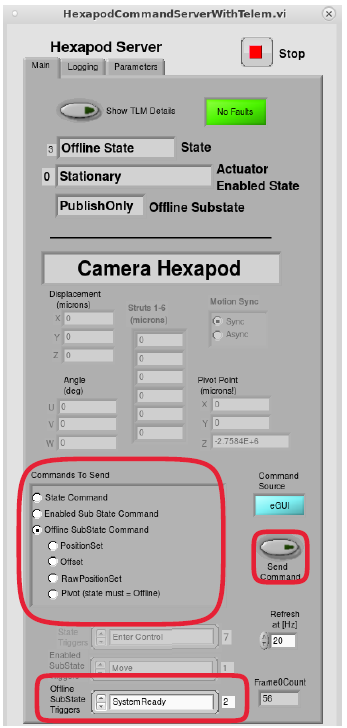
\includegraphics[width=1.79167in]{jira_imgs/1024.png}

\medskip }
\end{minipage}
\\ \cdashline{2-2}


 & Expected Result \\
 & \begin{minipage}[t]{15cm}{\footnotesize
The system transitions from the OfflineState/PublishOnly substate to the
OfflineState/AvailableState substate and the Command Source says
eGUI.\\[2\baselineskip]

\medskip }
\end{minipage} \\ \cdashline{2-2}

 & Actual Result \\
 & \begin{minipage}[t]{15cm}{\footnotesize
We transited the system to the OfflineState/AvailableState substate.

\medskip }
\end{minipage} \\ \cdashline{2-2}

 & Status: \textbf{ Initial Pass } \\ \hline

4 & Description \\
 & \begin{minipage}[t]{15cm}
{\footnotesize
\textbf{OFFLINESTATE -\textgreater{} STANDBYSTATE}\\
Click on the State Command field in the Commands to Send section.\\
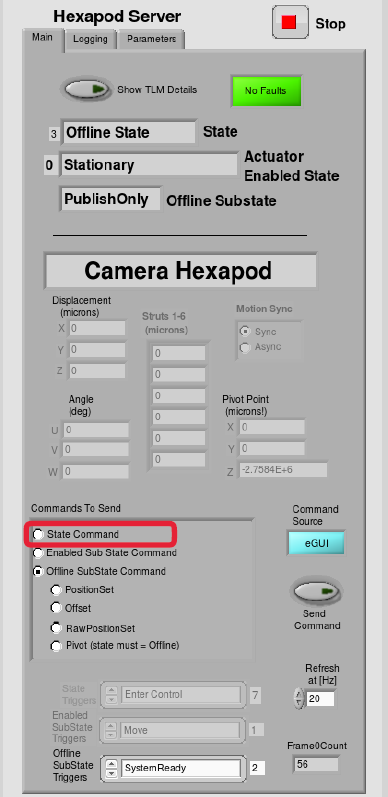
\includegraphics[width=1.79167in]{jira_imgs/1028.png}

\medskip }
\end{minipage}
\\ \cdashline{2-2}


 & Expected Result \\
 & \begin{minipage}[t]{15cm}{\footnotesize
The State Triggers dialogue box shown below becomes visible.\\
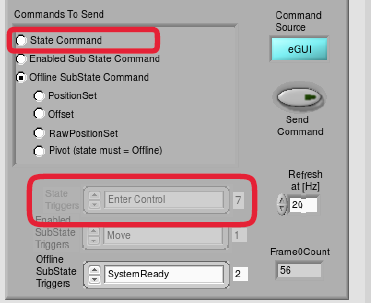
\includegraphics[width=1.79167in]{jira_imgs/1029.png}

\medskip }
\end{minipage} \\ \cdashline{2-2}

 & Actual Result \\
 & \begin{minipage}[t]{15cm}{\footnotesize
We transited the system to the Standby state.

\medskip }
\end{minipage} \\ \cdashline{2-2}

 & Status: \textbf{ Initial Pass } \\ \hline

5 & Description \\
 & \begin{minipage}[t]{15cm}
{\footnotesize
Scroll through the available trigger options to select ``Enter Control''
and click the Send Command button.

\medskip }
\end{minipage}
\\ \cdashline{2-2}


 & Expected Result \\
 & \begin{minipage}[t]{15cm}{\footnotesize
The system transitions to the Standby state and the primary state
display box at the top of the Main says Standby State.

\medskip }
\end{minipage} \\ \cdashline{2-2}

 & Actual Result \\
 & \begin{minipage}[t]{15cm}{\footnotesize
We transited the system to the Standby state.

\medskip }
\end{minipage} \\ \cdashline{2-2}

 & Status: \textbf{ Initial Pass } \\ \hline

6 & Description \\
 & \begin{minipage}[t]{15cm}
{\footnotesize
\textbf{STANDBYSTATE -\textgreater{} DISABLEDSTATE}\\
From the StandbyState, send a Start State command.

\medskip }
\end{minipage}
\\ \cdashline{2-2}


 & Expected Result \\
 & \begin{minipage}[t]{15cm}{\footnotesize
The system transitions into DisabledState and the current configuration
parameters are maintained from the default parameters or from the
previous DDS start command.~

\medskip }
\end{minipage} \\ \cdashline{2-2}

 & Actual Result \\
 & \begin{minipage}[t]{15cm}{\footnotesize
We transited the system to the Disabled state.

\medskip }
\end{minipage} \\ \cdashline{2-2}

 & Status: \textbf{ Initial Pass } \\ \hline

7 & Description \\
 & \begin{minipage}[t]{15cm}
{\footnotesize
\textbf{DISABLEDSTATE -\textgreater{} ENABLEDSTATE}\\
From the DisabledState, send an Enable State Command.~

\medskip }
\end{minipage}
\\ \cdashline{2-2}


 & Expected Result \\
 & \begin{minipage}[t]{15cm}{\footnotesize
The system transitions into the EnabledState/Stationary substate, the
motor drives are enabled and and motion can be commanded.~

\medskip }
\end{minipage} \\ \cdashline{2-2}

 & Actual Result \\
 & \begin{minipage}[t]{15cm}{\footnotesize
We transited the system to the Enabled state.

\medskip }
\end{minipage} \\ \cdashline{2-2}

 & Status: \textbf{ Initial Pass } \\ \hline

8 & Description \\
 & \begin{minipage}[t]{15cm}
{\footnotesize
\textless{}conditional state\textgreater{}\\
\textbf{FAULTSTATE}\\
If a Fault occurs in any of the other states, the system will
automatically transition to the Fault State. While in the Fault state,
send a clearError.\\
Note: If the fault that occurs goes through the interlock system, reset
the safety relay switch and send a clearError command.

\medskip }
\end{minipage}
\\ \cdashline{2-2}


 & Expected Result \\
 & \begin{minipage}[t]{15cm}{\footnotesize
The system transitions back to the OfflineState/PublishOnly substate.
(Go back to Step 3)

\medskip }
\end{minipage} \\ \cdashline{2-2}

 & Actual Result \\
 & \begin{minipage}[t]{15cm}{\footnotesize
For the safety interlock, press the E-stop first, click the switch
button of release interlock 2, release the E-stop, click the switch
button of reset interlock. By doing this, we could put/ release the
safety interlock. No clearError in software side is
needed.\\[2\baselineskip]When we opened the hexapod GUI, there was the
simulink error after hitting the systemReady command and entered the
Fault state. We can use the clearError to leave the Fault state and do
the state transitions.

\medskip }
\end{minipage} \\ \cdashline{2-2}

 & Status: \textbf{ Initial Pass } \\ \hline

9 & Description \\
 & \begin{minipage}[t]{15cm}
{\footnotesize
\textbf{Follow \emph{3.3.1 Positioning} of the LSST Hexapods-Rotator
Acceptance Test Procedure, Sheet 23-24.}

\medskip }
\end{minipage}
\\ \cdashline{2-2}

 & Test Data \\
 & \begin{minipage}[t]{15cm}{\footnotesize
\textbf{Deviation:~}Test this with no performance payload and at a
single elevation angle of zero degrees.

\medskip }
\end{minipage} \\ \cdashline{2-2}

 & Expected Result \\
 & \begin{minipage}[t]{15cm}{\footnotesize
The position of the hexapod is able to be commanded and no software
limits or limit switches are tripped.

\medskip }
\end{minipage} \\ \cdashline{2-2}

 & Actual Result \\
 & \begin{minipage}[t]{15cm}{\footnotesize
Measurements for the positioning could not be completed due to a failure
in drive \#3.\\
1) The tilt angle, tilt offset distance and pivot distance are all OK,
but once reached, the X and Zdon't seem to be able to reach position to
within \textasciitilde{}2mm\\
2) Laser tracker seems to contradict MOOG's statement about corners
representing different combinations of the maximum simultaneous range
requirements for X and Z

\medskip }
\end{minipage} \\ \cdashline{2-2}

 & Issues found executing this step:  \\
 & \begin{minipage}[t]{13cm}{\footnotesize
\href{https://jira.lsstcorp.org/browse/FRACAS-28}{FRACAS-28}~~Camera Hexapod Drive \#3 Failure

\medskip }
\end{minipage} \\ \cdashline{2-2}
 & Status: \textbf{ Fail } \\ \hline

10 & Description \\
 & \begin{minipage}[t]{15cm}
{\footnotesize
\textbf{Follow \emph{3.3.2 Centers of Rotation} of the LSST
Hexapods-Rotator Acceptance Test Procedure, Sheet 24-25.}

\medskip }
\end{minipage}
\\ \cdashline{2-2}

 & Test Data \\
 & \begin{minipage}[t]{15cm}{\footnotesize
\textbf{Deviation:~}Record pivot position through the EUI.

\medskip }
\end{minipage} \\ \cdashline{2-2}

 & Expected Result \\
 & \begin{minipage}[t]{15cm}{\footnotesize
The center of rotation is able to be moved.

\medskip }
\end{minipage} \\ \cdashline{2-2}

 & Actual Result \\
 & \begin{minipage}[t]{15cm}{\footnotesize
\emph{COR at 1.938m from the rotator to camera interface}\\
Laser tracker-determined COR: 1930+/-8.2{[}mm{]}\\
\emph{COR at the rotator to camera interface}\\
Laser tracker-determined COR: set value COR 33.75{[}mm{]}; SA measured =
923+/-1 {[}mm{]}\\
Complies with requirement with caveat that there is an offset at the
rotatorsurface: 820.4mm

\medskip }
\end{minipage} \\ \cdashline{2-2}

 & Status: \textbf{ Initial Pass } \\ \hline

11 & Description \\
 & \begin{minipage}[t]{15cm}
{\footnotesize
\textbf{Follow \emph{3.3.3 Cross-Talk Motion~}of the LSST
Hexapods-Rotator Acceptance Test Procedure, Sheet 25.}

\medskip }
\end{minipage}
\\ \cdashline{2-2}


 & Expected Result \\
 & \begin{minipage}[t]{15cm}{\footnotesize
There is no cross-talk observed (actuator positioning errors and
erroneous geometry are minimal)

\medskip }
\end{minipage} \\ \cdashline{2-2}

 & Actual Result \\
 & \begin{minipage}[t]{15cm}{\footnotesize
Based on rest of tests

\medskip }
\end{minipage} \\ \cdashline{2-2}

 & Status: \textbf{ Initial Pass } \\ \hline

12 & Description \\
 & \begin{minipage}[t]{15cm}
{\footnotesize
\textbf{Follow \emph{3.3.4 Radial (X and Y) Translational Range~}of the
LSST Hexapods-Rotator Acceptance Test Procedure, Sheet 25.}

\medskip }
\end{minipage}
\\ \cdashline{2-2}

 & Test Data \\
 & \begin{minipage}[t]{15cm}{\footnotesize
\textbf{Deviation:~}Only test at a zero degree elevation angle.

\medskip }
\end{minipage} \\ \cdashline{2-2}

 & Expected Result \\
 & \begin{minipage}[t]{15cm}{\footnotesize
The hexapod is capable of moving to the positions in the XY plane listed
in the Acceptance Test Procedure.

\medskip }
\end{minipage} \\ \cdashline{2-2}

 & Actual Result \\
 & \begin{minipage}[t]{15cm}{\footnotesize
1. 7.57428275,0,0,0,0,0\\
2. 5.3578403, 5.37473926,0,0,0,0\\
3. 0,7.58852237,0,0,0,0\\
4. -5.34249993, 5.33297113,0,0,0,0\\
5. -7.57839578,0,0,0,0,0\\
6. -5.34249993, -5.38597352,0,0,0,0\\
7. 0;-7.55189491,0,0,0,0\\
8. 5.3578403; -5.34205358;0;0;0;0

\medskip }
\end{minipage} \\ \cdashline{2-2}

 & Status: \textbf{ Initial Pass } \\ \hline

13 & Description \\
 & \begin{minipage}[t]{15cm}
{\footnotesize
\textbf{Follow \emph{3.3.6 Axial (Z) Translation Range~}of the LSST
Hexapods-Rotator Acceptance Test Procedure, Sheet 27.}

\medskip }
\end{minipage}
\\ \cdashline{2-2}

 & Test Data \\
 & \begin{minipage}[t]{15cm}{\footnotesize
\textbf{Deviation:~}Only test at a zero degree elevation angle.

\medskip }
\end{minipage} \\ \cdashline{2-2}

 & Expected Result \\
 & \begin{minipage}[t]{15cm}{\footnotesize
The hexapod is capable of moving to the positions in the Z plane listed
in the Acceptance Test Procedure.~

\medskip }
\end{minipage} \\ \cdashline{2-2}

 & Actual Result \\
 & \begin{minipage}[t]{15cm}{\footnotesize
1. 0;0;8.72487391;0;0;0\\
2. 0,0, -8.710510168,0,0,0\\
3. 0;0;8.70619302;0;0;0

\medskip }
\end{minipage} \\ \cdashline{2-2}

 & Status: \textbf{ Initial Pass } \\ \hline

14 & Description \\
 & \begin{minipage}[t]{15cm}
{\footnotesize
\textbf{Follow \emph{3.3.8 Rotational Range Around X-Axis (Tip) and
Y-Axis (Tilt)~}of the LSST Hexapods-Rotator Acceptance Test Procedure,
Sheet 28-29.}

\medskip }
\end{minipage}
\\ \cdashline{2-2}

 & Test Data \\
 & \begin{minipage}[t]{15cm}{\footnotesize
\textbf{Deviation:~}Only test at a zero degree elevation angle.

\medskip }
\end{minipage} \\ \cdashline{2-2}

 & Expected Result \\
 & \begin{minipage}[t]{15cm}{\footnotesize
The hexapod is capable of moving to the positions in the RXRY plane
listed in the Acceptance Test Procedure.

\medskip }
\end{minipage} \\ \cdashline{2-2}

 & Actual Result \\
 & \begin{minipage}[t]{15cm}{\footnotesize
Command (0,0,0,0.24 deg,0,0): (0,0,0,0.2429,0,0)\\
Command (0,0,0,0.170deg,0.170deg,0): (0,0,0,0.1732,0.1707,0)\\
Command (0,0,0,0,0.24deg,0): (0,0,0,0.2402,0,0)\\
Command (0,0,0,-0.170deg,0.170deg,0): (0,0,0,-0.1689,0.1714,0)\\
Command (0,0,0,-0.24deg,0,0): (0,0,0,-0.2414,0,0)\\
Command (0,0,0,-0.170deg,-0.170deg,0): (0,0,0,-0.169,-0.1703,0)\\
Command (0,0,0,0,-0.24deg,0): (0,0,0,0,-0.2431,0)\\
Command (0,0,0,0.170deg,-0.170deg,0):
(0,0,0,0.173,-0.1714,0)\\[2\baselineskip]Measurements error
STDEV\textless{}0.00205Deg

\medskip }
\end{minipage} \\ \cdashline{2-2}

 & Status: \textbf{ Initial Pass } \\ \hline

15 & Description \\
 & \begin{minipage}[t]{15cm}
{\footnotesize
\textbf{Follow \emph{3.3.10 Rotation Range Around Z-Axis (Twist)~}of the
LSST Hexapods-Rotator Acceptance Test Procedure, Sheet 30.}

\medskip }
\end{minipage}
\\ \cdashline{2-2}

 & Test Data \\
 & \begin{minipage}[t]{15cm}{\footnotesize
\textbf{Deviation:~}Only test at a zero degree elevation angle.

\medskip }
\end{minipage} \\ \cdashline{2-2}

 & Expected Result \\
 & \begin{minipage}[t]{15cm}{\footnotesize
The hexapod is capable of moving to the positions in the RZ-axis listed
in the Acceptance Test Procedure.

\medskip }
\end{minipage} \\ \cdashline{2-2}

 & Actual Result \\
 & \begin{minipage}[t]{15cm}{\footnotesize
Command (0,0,0,0,0,0.1deg): (0,0,0,0,0,0.0999)\\
Command (0,0,0,0,0,-0.1deg): (0,0,0,0,0,-0.09955)\\[2\baselineskip]Error
\textless{} 0.015Deg

\medskip }
\end{minipage} \\ \cdashline{2-2}

 & Status: \textbf{ Initial Pass } \\ \hline

16 & Description \\
 & \begin{minipage}[t]{15cm}
{\footnotesize
\textbf{Follow \emph{3.3.12 Hexapod Repeatability} of the LSST
Hexapods-Rotato Acceptance Test Procedure, Sheet 31.}

\medskip }
\end{minipage}
\\ \cdashline{2-2}


 & Expected Result \\
 & \begin{minipage}[t]{15cm}{\footnotesize
The repeatability is as good as the test equipment can capture. This
means that the repeatability is limited by the resolution of the test
equipment.

\medskip }
\end{minipage} \\ \cdashline{2-2}

 & Actual Result \\
 & \begin{minipage}[t]{15cm}{\footnotesize

\medskip }
\end{minipage} \\ \cdashline{2-2}

 & Status: \textbf{ Not Executed } \\ \hline

17 & Description \\
 & \begin{minipage}[t]{15cm}
{\footnotesize
\textbf{Follow \emph{3.3.13 Hexapod Absolute Accuracy~}of the LSST
Hexapods-Rotator Acceptance Test Procedure, Sheet 38-42.}

\medskip }
\end{minipage}
\\ \cdashline{2-2}

 & Test Data \\
 & \begin{minipage}[t]{15cm}{\footnotesize
\textbf{Deviation:~}Only test at a zero degree elevation angle.

\medskip }
\end{minipage} \\ \cdashline{2-2}

 & Expected Result \\
 & \begin{minipage}[t]{15cm}{\footnotesize
The accuracy of the hexapod is good enough to be consistently repeated.

\medskip }
\end{minipage} \\ \cdashline{2-2}

 & Actual Result \\
 & \begin{minipage}[t]{15cm}{\footnotesize
Shall be done in test cases 12-15.

\medskip }
\end{minipage} \\ \cdashline{2-2}

 & Status: \textbf{ Initial Pass } \\ \hline

18 & Description \\
 & \begin{minipage}[t]{15cm}
{\footnotesize
\textbf{Follow \emph{3.3.16 Hexapod Radial (X and Y) and Axial (Z)
Velocity Range} and~\emph{3.3.17 Hexapod Rotational Velocity~}of the
LSST Hexapods-Rotator Acceptance Test Procedure, Sheet 43-44.}

\medskip }
\end{minipage}
\\ \cdashline{2-2}

 & Test Data \\
 & \begin{minipage}[t]{15cm}{\footnotesize
\textbf{Deviation:~}Only test this using synchronous mode.

\medskip }
\end{minipage} \\ \cdashline{2-2}

 & Expected Result \\
 & \begin{minipage}[t]{15cm}{\footnotesize
The hexapod velocity exceeds the 152um/s in XY and 0.0039deg/s in RXYRY
and RZ requirements.

\medskip }
\end{minipage} \\ \cdashline{2-2}

 & Actual Result \\
 & \begin{minipage}[t]{15cm}{\footnotesize
Hexapod meets requirements.

\medskip }
\end{minipage} \\ \cdashline{2-2}

 & Status: \textbf{ Initial Pass } \\ \hline

19 & Description \\
 & \begin{minipage}[t]{15cm}
{\footnotesize
\textbf{Follow \emph{3.3.18 Hexapod Heat Dissipation~}of the LSST
Hexapods-Rotator Acceptance Test Procedure, Sheet 44.}

\medskip }
\end{minipage}
\\ \cdashline{2-2}


 & Expected Result \\
 & \begin{minipage}[t]{15cm}{\footnotesize
The current measured by the inductive current probes is calculated to
meet the heat dissipation requirement.

\medskip }
\end{minipage} \\ \cdashline{2-2}

 & Actual Result \\
 & \begin{minipage}[t]{15cm}{\footnotesize
As this was originally tested with a surrogate mass, this step was left
unexecuted and will be tested in the future with ComCam (with load).~

\medskip }
\end{minipage} \\ \cdashline{2-2}

 & Status: \textbf{ Not Executed } \\ \hline

\end{longtable}

\paragraph{ LVV-T1599 - Camera Hexapod Software Functional Re-verification }\mbox{}\\

Version \textbf{1}.
Open  \href{https://jira.lsstcorp.org/secure/Tests.jspa#/testCase/LVV-T1599}{\textit{ LVV-T1599 } }
test case in Jira.

The objective of this test case is to re-verify the functional
requirements of the camera hexapod's software, after shipment of the
hardware from the vendor's facility to the Summit, as defined in \citeds{LTS-206}
and \citeds{LTS-160}. This test case will only exercise the functionality that
was executed previously and meets the following criteria:

\begin{itemize}
\tightlist
\item
  Only requires the camera hexapod to be operable
\item
  Only requires testing of the synchronous mode

  \begin{itemize}
  \tightlist
  \item
    \textbf{Asynchronous mode is not a standard mode of operation}
  \end{itemize}
\item
  Only requires the vendors EUI software and hardware via local control

  \begin{itemize}
  \tightlist
  \item
    Does \textbf{NOT} require integration with SAL
  \end{itemize}
\item
  Does \textbf{NOT} require the camera hexapod to be loaded with the
  camera simulated mass or actual camera hardware
\end{itemize}

The software functional requirements were previously verified during the
test campaign by the vendor at the vendor's facility and accepted by
LSST during the Factory Acceptance Test review. The test procedure used
during the vendor's acceptance testing is the \emph{LSST
Hexapods-Rotator Software Acceptance Test Procedure} which is attached
to this test case. The test steps of this test case are taken directly
from that document on how to perform the test in a similar way as was
performed previously and includes changes noted by the
vendor.\\[2\baselineskip]See the attached \emph{LSST Hexapod Operator's
Manual} for more information on how to operate the hexapod.

\textbf{ Preconditions}:\\
Prior to the execution of this test case to re-verify the Camera Hexapod
hardware functional requirements, the following Summit tasks must be
completed:

\begin{itemize}
\tightlist
\item
  The Hexapod has been installed on the camera cart

  \begin{itemize}
  \tightlist
  \item
    \url{https://jira.lsstcorp.org/browse/SUMMIT-3224}
  \end{itemize}
\item
  The Hexapod Controller has been deployed on the summit

  \begin{itemize}
  \tightlist
  \item
    \url{https://jira.lsstcorp.org/browse/SUMMIT-3229}
  \end{itemize}
\item
  Boxes for the Hexapod have been transported to the 3rd level

  \begin{itemize}
  \tightlist
  \item
    \url{https://jira.lsstcorp.org/browse/SUMMIT-3230}
  \end{itemize}
\item
  All Hexapod cables and cabinets have been prepared for integration
  with camera cart

  \begin{itemize}
  \tightlist
  \item
    \url{https://jira.lsstcorp.org/browse/SUMMIT-3231}
  \end{itemize}
\item
  The offset has been installed onto the integrating structure

  \begin{itemize}
  \tightlist
  \item
    \url{https://jira.lsstcorp.org/browse/SUMMIT-3293}
  \end{itemize}
\item
  The Camera Hexapod electrical connections have been tested

  \begin{itemize}
  \tightlist
  \item
    \url{https://jira.lsstcorp.org/browse/SUMMIT-3294}
  \end{itemize}
\end{itemize}

Execution status: {\bf Initial Pass }

Final comment:\\


Detailed steps results:

\begin{longtable}{p{1cm}p{15cm}}
\hline
{Step} & Step Details\\ \hline
1 & Description \\
 & \begin{minipage}[t]{15cm}
{\footnotesize
\textbf{STARTING THE EUI}\\[2\baselineskip]Double click the Hexapod GUI
Viewer desktop icon on the computer.

\begin{itemize}
\tightlist
\item
  This can be done on the Dell Management PC or another computer on the
  same network
\end{itemize}

\medskip }
\end{minipage}
\\ \cdashline{2-2}


 & Expected Result \\
 & \begin{minipage}[t]{15cm}{\footnotesize
A prompt to enter the password is shown.

\medskip }
\end{minipage} \\ \cdashline{2-2}

 & Actual Result \\
 & \begin{minipage}[t]{15cm}{\footnotesize
We saw the prompt window and asked for the password.

\medskip }
\end{minipage} \\ \cdashline{2-2}

 & Status: \textbf{ Initial Pass } \\ \hline

2 & Description \\
 & \begin{minipage}[t]{15cm}
{\footnotesize
Enter the password ``lsst-vnc''

\begin{itemize}
\tightlist
\item
  If the EUI isn't automatically up and running when the VNC opens,
  double click on the Hexapod-eGUI icon on the VNC viewer
\end{itemize}

\medskip }
\end{minipage}
\\ \cdashline{2-2}


 & Expected Result \\
 & \begin{minipage}[t]{15cm}{\footnotesize
The EUI is in the Offline State/PublishOnly substate and is able to
publish through SAL but cannot receive commands.

\medskip }
\end{minipage} \\ \cdashline{2-2}

 & Actual Result \\
 & \begin{minipage}[t]{15cm}{\footnotesize
After we entered the ``lsst-vnc'', we can log in the system. The initial
state is Offline State/PublishOnly. We saw the green light of DDS
connected.

\medskip }
\end{minipage} \\ \cdashline{2-2}

 & Status: \textbf{ Initial Pass } \\ \hline

3 & Description \\
 & \begin{minipage}[t]{15cm}
{\footnotesize
\textbf{OFFLINESTATE/AVAILABLESTATE}\\
On the Main tab, select the ``Offline SubState Cmd'' field in the
Commands to Send section, set the Offline SubState Triggers to ``System
Ready'' and click on the Send Command button.\\
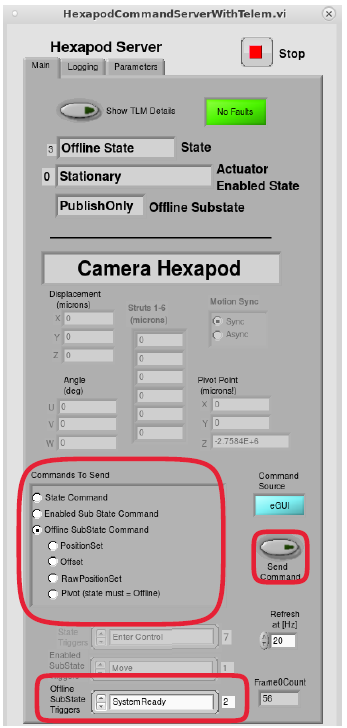
\includegraphics[width=1.79167in]{jira_imgs/1024.png}

\medskip }
\end{minipage}
\\ \cdashline{2-2}


 & Expected Result \\
 & \begin{minipage}[t]{15cm}{\footnotesize
The system transitions from the OfflineState/PublishOnly substate to the
OfflineState/AvailableState substate and the Command Source says
eGUI.\\[2\baselineskip]

\medskip }
\end{minipage} \\ \cdashline{2-2}

 & Actual Result \\
 & \begin{minipage}[t]{15cm}{\footnotesize
We transited the system to the OfflineState/AvailableState substate.

\medskip }
\end{minipage} \\ \cdashline{2-2}

 & Status: \textbf{ Initial Pass } \\ \hline

4 & Description \\
 & \begin{minipage}[t]{15cm}
{\footnotesize
\textbf{OFFLINESTATE -\textgreater{} STANDBYSTATE}\\
Click on the State Command field in the Commands to Send section.\\
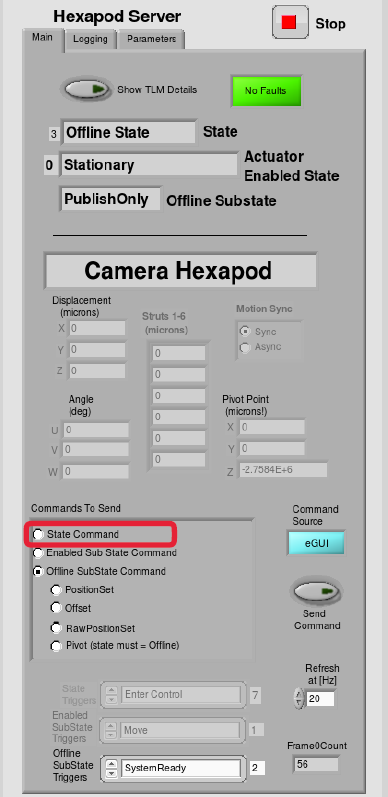
\includegraphics[width=1.79167in]{jira_imgs/1028.png}

\medskip }
\end{minipage}
\\ \cdashline{2-2}


 & Expected Result \\
 & \begin{minipage}[t]{15cm}{\footnotesize
The State Triggers dialogue box shown below becomes visible.\\
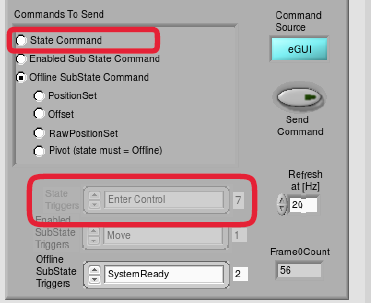
\includegraphics[width=1.79167in]{jira_imgs/1029.png}

\medskip }
\end{minipage} \\ \cdashline{2-2}

 & Actual Result \\
 & \begin{minipage}[t]{15cm}{\footnotesize
We transited the system to the Standby state.

\medskip }
\end{minipage} \\ \cdashline{2-2}

 & Status: \textbf{ Initial Pass } \\ \hline

5 & Description \\
 & \begin{minipage}[t]{15cm}
{\footnotesize
Scroll through the available trigger options to select ``Enter Control''
and click the Send Command button.

\medskip }
\end{minipage}
\\ \cdashline{2-2}


 & Expected Result \\
 & \begin{minipage}[t]{15cm}{\footnotesize
The system transitions to the Standby state and the primary state
display box at the top of the Main says Standby State.

\medskip }
\end{minipage} \\ \cdashline{2-2}

 & Actual Result \\
 & \begin{minipage}[t]{15cm}{\footnotesize
We transited the system to the Standby state.

\medskip }
\end{minipage} \\ \cdashline{2-2}

 & Status: \textbf{ Initial Pass } \\ \hline

6 & Description \\
 & \begin{minipage}[t]{15cm}
{\footnotesize
\textbf{STANDBYSTATE -\textgreater{} DISABLEDSTATE}\\
From the StandbyState, send a Start State command.

\medskip }
\end{minipage}
\\ \cdashline{2-2}


 & Expected Result \\
 & \begin{minipage}[t]{15cm}{\footnotesize
The system transitions into DisabledState and the current configuration
parameters are maintained from the default parameters or from the
previous DDS start command.~

\medskip }
\end{minipage} \\ \cdashline{2-2}

 & Actual Result \\
 & \begin{minipage}[t]{15cm}{\footnotesize
Duplication of the test case 6 in LVV-T1598.

\medskip }
\end{minipage} \\ \cdashline{2-2}

 & Status: \textbf{ Initial Pass } \\ \hline

7 & Description \\
 & \begin{minipage}[t]{15cm}
{\footnotesize
\textbf{DISABLEDSTATE -\textgreater{} ENABLEDSTATE}\\
From the DisabledState, send an Enable State Command.~

\medskip }
\end{minipage}
\\ \cdashline{2-2}


 & Expected Result \\
 & \begin{minipage}[t]{15cm}{\footnotesize
The system transitions into the EnabledState/Stationary substate, the
motor drives are enabled and and motion can be commanded.~

\medskip }
\end{minipage} \\ \cdashline{2-2}

 & Actual Result \\
 & \begin{minipage}[t]{15cm}{\footnotesize
We transited the system to the Disabled state.

\medskip }
\end{minipage} \\ \cdashline{2-2}

 & Status: \textbf{ Initial Pass } \\ \hline

8 & Description \\
 & \begin{minipage}[t]{15cm}
{\footnotesize
\textless{}conditional state\textgreater{}\\
\textbf{FAULTSTATE}\\
If a Fault occurs in any of the other states, the system will
automatically transition to the Fault State. While in the Fault state,
send a clearError.\\
Note: If the fault that occurs goes through the interlock system, reset
the safety relay switch and send a clearError command.

\medskip }
\end{minipage}
\\ \cdashline{2-2}


 & Expected Result \\
 & \begin{minipage}[t]{15cm}{\footnotesize
The system transitions back to the OfflineState/PublishOnly substate.
(Go back to Step 3)

\medskip }
\end{minipage} \\ \cdashline{2-2}

 & Actual Result \\
 & \begin{minipage}[t]{15cm}{\footnotesize
For the safety interlock, press the E-top first, click the switch button
of release interlock 2, release the E-stop, click the switch button of
reset interlock. By doing this, we could put/ release the safety
interlock. No clearError in software side is
needed.\\[2\baselineskip]When we opened the hexapod GUI, there was the
simulink error after hitting the systemReady command and entered the
Fault state. We can use the clearError to leave the Fault state and do
the state transitions.

\medskip }
\end{minipage} \\ \cdashline{2-2}

 & Status: \textbf{ Initial Pass } \\ \hline

9 & Description \\
 & \begin{minipage}[t]{15cm}
{\footnotesize
\textbf{Section 3.1.1 of the attached Software Acceptance Test
Procedure\\
Test Sequence \#1 - Synchronous PositionSet and Move
Commands}\\[2\baselineskip]With the synchronous button enabled and in
enabled/stationary state, send a positionSet command of (0um, 0um,
200um, 0 deg, 0 deg, 0 deg) using the EUI.

\medskip }
\end{minipage}
\\ \cdashline{2-2}


 & Expected Result \\
 & \begin{minipage}[t]{15cm}{\footnotesize
The hexapod doesn't move.

\medskip }
\end{minipage} \\ \cdashline{2-2}

 & Actual Result \\
 & \begin{minipage}[t]{15cm}{\footnotesize
We sent the positionSet command of (0um, 0um, 200um, 0 deg, 0 deg, 0
deg) only and the hexapod did not move.

\medskip }
\end{minipage} \\ \cdashline{2-2}

 & Status: \textbf{ Initial Pass } \\ \hline

10 & Description \\
 & \begin{minipage}[t]{15cm}
{\footnotesize
With the synchronous button enabled and in enabled/stationary state,
send a positionSet command of (2000um, -3500um, 200um, .01 deg, -.05deg,
.002deg) using the EUI.

\medskip }
\end{minipage}
\\ \cdashline{2-2}


 & Expected Result \\
 & \begin{minipage}[t]{15cm}{\footnotesize
The hexapod doesn't move.

\medskip }
\end{minipage} \\ \cdashline{2-2}

 & Actual Result \\
 & \begin{minipage}[t]{15cm}{\footnotesize
We sent the positionSet command of (2000um, -3500um, 200um, .01 deg,
-.05deg, .002deg) only and the hexapod did not move.

\medskip }
\end{minipage} \\ \cdashline{2-2}

 & Status: \textbf{ Initial Pass } \\ \hline

11 & Description \\
 & \begin{minipage}[t]{15cm}
{\footnotesize
Send a move command using the EUI.

\medskip }
\end{minipage}
\\ \cdashline{2-2}


 & Expected Result \\
 & \begin{minipage}[t]{15cm}{\footnotesize
The hexapod moves to the last commanded position of (2000um, -3500um,
200um, .01 deg, -.05deg, .002deg) and the actuators complete the move at
nearly the same time as seen on the motion complete lights on the
telemetry screen.

\medskip }
\end{minipage} \\ \cdashline{2-2}

 & Actual Result \\
 & \begin{minipage}[t]{15cm}{\footnotesize
We saw the movement of hexapod with position (2000um, -3500um, 200um,
.01 deg, -.05deg, .002deg) after hitting the move command. The final
position is (1999um, -3500um, 200um, .01 deg, -.05deg, .002deg) on GUI.
We saw a ``1 um'' difference in x position.

\medskip }
\end{minipage} \\ \cdashline{2-2}

 & Status: \textbf{ Initial Pass } \\ \hline

12 & Description \\
 & \begin{minipage}[t]{15cm}
{\footnotesize
\textbf{Section 3.1.1 of the attached Software Acceptance Test
Procedure\\
Test Sequence \#2 - Pivot, PositionSet and Move
Commands}\\[2\baselineskip]In enabled/stationary state and at the last
commanded position of (2000um, -3500um, 200um, .01 deg, -.05deg,
.002deg), change the pivot point from the default location to (0,0,0)
using the EUI.

\medskip }
\end{minipage}
\\ \cdashline{2-2}


 & Expected Result \\
 & \begin{minipage}[t]{15cm}{\footnotesize
The actuator positions do not change, but the hexapod position is
(-407um, -3982um, 199um, 0.01deg, -0.05deg, 0.002deg)

\medskip }
\end{minipage} \\ \cdashline{2-2}

 & Actual Result \\
 & \begin{minipage}[t]{15cm}{\footnotesize
The default pivot position is (0, 0, -2758400um). Change the pivot to
(0, 0, 0) in the offline state (it can not be changed in the enabled
state). The hexapod position is (-408um, -3982um, 199um, 0.01deg,
-0.05deg, 0.002deg). The x position differs by 1 um from the case
11.\\[2\baselineskip]PS. The pivot value can only be changed in the
offline state not enabled/stationary state. There will be a prompt
window to complain the wrong state.

\medskip }
\end{minipage} \\ \cdashline{2-2}

 & Status: \textbf{ Initial Pass } \\ \hline

13 & Description \\
 & \begin{minipage}[t]{15cm}
{\footnotesize
In the enabled/stationary state, send a positionSet command of (2000um,
-3500um, 200um, .01 deg, -.05deg, .002deg) using the EUI.

\medskip }
\end{minipage}
\\ \cdashline{2-2}


 & Expected Result \\
 & \begin{minipage}[t]{15cm}{\footnotesize
The hexapod doesn't move.

\medskip }
\end{minipage} \\ \cdashline{2-2}

 & Actual Result \\
 & \begin{minipage}[t]{15cm}{\footnotesize
We sent the positionSet command of (2000um, -3500um, 200um, .01 deg,
-.05deg, .002deg) only and the hexapod did not move.

\medskip }
\end{minipage} \\ \cdashline{2-2}

 & Status: \textbf{ Initial Pass } \\ \hline

14 & Description \\
 & \begin{minipage}[t]{15cm}
{\footnotesize
Send a move command using the EUI.

\medskip }
\end{minipage}
\\ \cdashline{2-2}


 & Expected Result \\
 & \begin{minipage}[t]{15cm}{\footnotesize
The hexapod moves to the commanded position of (2000um, -3500um, 200um,
.01 deg, -.05deg, .002deg) and the actuators change position to account
for the new pivot point.

\medskip }
\end{minipage} \\ \cdashline{2-2}

 & Actual Result \\
 & \begin{minipage}[t]{15cm}{\footnotesize
The hexapod moved to the position of (2000um, -3500um, 200um, .01 deg,
-.05deg, .002deg) based on GUI with the new pivot point.

\medskip }
\end{minipage} \\ \cdashline{2-2}

 & Status: \textbf{ Initial Pass } \\ \hline

15 & Description \\
 & \begin{minipage}[t]{15cm}
{\footnotesize
\textbf{Section 3.1.1 of the attached Software Acceptance Test
Procedure\\
Test Sequence \#4 - Synchronous Offset and Move
Commands}\\[2\baselineskip]With the synchronous button enabled and in
enabled/stationary state, send a positionSet command of (500um, 800um,
200um, 0 deg, 0 deg, 0 deg).

\medskip }
\end{minipage}
\\ \cdashline{2-2}


 & Expected Result \\
 & \begin{minipage}[t]{15cm}{\footnotesize
The hexapod doesn't move.

\medskip }
\end{minipage} \\ \cdashline{2-2}

 & Actual Result \\
 & \begin{minipage}[t]{15cm}{\footnotesize
We sent the positionSet command of (500um, 800um, 200um, 0 deg, 0 deg, 0
deg) only and the hexapod did not move.

\medskip }
\end{minipage} \\ \cdashline{2-2}

 & Status: \textbf{ Initial Pass } \\ \hline

16 & Description \\
 & \begin{minipage}[t]{15cm}
{\footnotesize
With the synchronous button enabled and in enabled/stationary state,
send an offset command of (0um, 0um, 2000um, 0 deg, 0 deg, 0 deg).~

\medskip }
\end{minipage}
\\ \cdashline{2-2}


 & Expected Result \\
 & \begin{minipage}[t]{15cm}{\footnotesize
The hexapod doesn't move.

\medskip }
\end{minipage} \\ \cdashline{2-2}

 & Actual Result \\
 & \begin{minipage}[t]{15cm}{\footnotesize
We sent the offset command of (0um, 0um, 2000um, 0 deg, 0 deg, 0 deg)
only and the hexapod did not move.

\medskip }
\end{minipage} \\ \cdashline{2-2}

 & Status: \textbf{ Initial Pass } \\ \hline

17 & Description \\
 & \begin{minipage}[t]{15cm}
{\footnotesize
Send a move command.

\medskip }
\end{minipage}
\\ \cdashline{2-2}


 & Expected Result \\
 & \begin{minipage}[t]{15cm}{\footnotesize
The hexapod moves only 2000um in Z from the previous position and the
actuators complete the move at nearly the same time as seen on the
motion complete lights on the telemetry screen.

\medskip }
\end{minipage} \\ \cdashline{2-2}

 & Actual Result \\
 & \begin{minipage}[t]{15cm}{\footnotesize
Put the hexapod to origin. Do the case 15 and 16 and move. The hexapod
moves to (1um, 0, 2000um, 0, 0, 0). We saw the offset command will
override the positionSet command from case 15.

\medskip }
\end{minipage} \\ \cdashline{2-2}

 & Status: \textbf{ Initial Pass } \\ \hline

18 & Description \\
 & \begin{minipage}[t]{15cm}
{\footnotesize
\textbf{Instead of Asynchronous Test}\\
{With the synchronous button enabled and in enabled/stationary
state,}{\textbf{~}}{s}end a position set command of (0um, 0um, 0um,
0.1deg, 0deg, 0deg)

\medskip }
\end{minipage}
\\ \cdashline{2-2}


 & Expected Result \\
 & \begin{minipage}[t]{15cm}{\footnotesize
The hexapod doesn't move.

\medskip }
\end{minipage} \\ \cdashline{2-2}

 & Actual Result \\
 & \begin{minipage}[t]{15cm}{\footnotesize
We sent the positionSet command of (0, 0, 0, 0.1deg, 0, 0) only and the
hexapod did not move.

\medskip }
\end{minipage} \\ \cdashline{2-2}

 & Status: \textbf{ Initial Pass } \\ \hline

19 & Description \\
 & \begin{minipage}[t]{15cm}
{\footnotesize
Send a move command.

\medskip }
\end{minipage}
\\ \cdashline{2-2}


 & Expected Result \\
 & \begin{minipage}[t]{15cm}{\footnotesize
The hexapod moves to the commanded position of (0um, 0um, 0um, 0.1deg,
0deg, 0deg)

\medskip }
\end{minipage} \\ \cdashline{2-2}

 & Actual Result \\
 & \begin{minipage}[t]{15cm}{\footnotesize
1. The hexapod moved to (0 , -2um, 0, 0.1deg, 0, 0) based on GUI from
the (1um, 0, 2000um, 0, 0, 0) in case 17.\\
2. The hexapod moved to (0 , 1um, 0, 0.1deg, 0, 0) based on GUI from the
origin (0, -1um, 0, 0, 0, 0).

\medskip }
\end{minipage} \\ \cdashline{2-2}

 & Status: \textbf{ Initial Pass } \\ \hline

20 & Description \\
 & \begin{minipage}[t]{15cm}
{\footnotesize
With the synchronous button enabled and in enabled/stationary
state,\textbf{~}send a position set command of (0um, 0um, 0um, 0deg,
0.1deg, 0deg)

\medskip }
\end{minipage}
\\ \cdashline{2-2}


 & Expected Result \\
 & \begin{minipage}[t]{15cm}{\footnotesize
The hexapod doesn't move.

\medskip }
\end{minipage} \\ \cdashline{2-2}

 & Actual Result \\
 & \begin{minipage}[t]{15cm}{\footnotesize
We sent the positionSet command of (0, 0, 0, 0, 0.1deg, 0) only and the
hexapod did not move.

\medskip }
\end{minipage} \\ \cdashline{2-2}

 & Status: \textbf{ Initial Pass } \\ \hline

21 & Description \\
 & \begin{minipage}[t]{15cm}
{\footnotesize
Send a move command.

\medskip }
\end{minipage}
\\ \cdashline{2-2}


 & Expected Result \\
 & \begin{minipage}[t]{15cm}{\footnotesize
The hexapod moves to the commanded position of (0um, 0um, 0um, 0deg,
0.1deg, 0deg)

\medskip }
\end{minipage} \\ \cdashline{2-2}

 & Actual Result \\
 & \begin{minipage}[t]{15cm}{\footnotesize
The hexapod moved to (0 , -1um, 0, 0, 0.1deg, 0) based on GUI from the
origin (0, -1um, 0, 0, 0, 0).

\medskip }
\end{minipage} \\ \cdashline{2-2}

 & Status: \textbf{ Initial Pass } \\ \hline

22 & Description \\
 & \begin{minipage}[t]{15cm}
{\footnotesize
With the synchronous button enabled and in enabled/stationary
state,\textbf{~}send a position set command of (0um, 0um, 0um, 0.1deg,
0.1deg, 0deg)

\medskip }
\end{minipage}
\\ \cdashline{2-2}


 & Expected Result \\
 & \begin{minipage}[t]{15cm}{\footnotesize
The hexapod doesn't move.

\medskip }
\end{minipage} \\ \cdashline{2-2}

 & Actual Result \\
 & \begin{minipage}[t]{15cm}{\footnotesize
We sent the positionSet command of (0, 0, 0, 0.1deg, 0.1deg, 0) only and
the hexapod did not move.

\medskip }
\end{minipage} \\ \cdashline{2-2}

 & Status: \textbf{ Initial Pass } \\ \hline

23 & Description \\
 & \begin{minipage}[t]{15cm}
{\footnotesize
Send a move command.

\medskip }
\end{minipage}
\\ \cdashline{2-2}


 & Expected Result \\
 & \begin{minipage}[t]{15cm}{\footnotesize
The hexapod moves to the commanded position of (0um, 0um, 0um, 0.1deg,
0.1deg, 0deg)

\medskip }
\end{minipage} \\ \cdashline{2-2}

 & Actual Result \\
 & \begin{minipage}[t]{15cm}{\footnotesize
The hexapod moved to (0 , 0, 0, 0.1deg, 0.1deg, 0) based on GUI from the
origin (0, 0, 0, 0, 0, 0).

\medskip }
\end{minipage} \\ \cdashline{2-2}

 & Status: \textbf{ Initial Pass } \\ \hline

24 & Description \\
 & \begin{minipage}[t]{15cm}
{\footnotesize
\textbf{Section 3.1.1 of the attached Software Acceptance Test
Procedure\\
Test Sequence \#5 - Stop Commands}\\[2\baselineskip]In
enabled/stationary state, send a position set command of (0um, 0um,
5000um, 0 deg, 0 deg, 0 deg).

\medskip }
\end{minipage}
\\ \cdashline{2-2}


 & Expected Result \\
 & \begin{minipage}[t]{15cm}{\footnotesize
The hexapod doesn't move.

\medskip }
\end{minipage} \\ \cdashline{2-2}

 & Actual Result \\
 & \begin{minipage}[t]{15cm}{\footnotesize
We sent the positionSet command of (0, 0, 5000um, 0, 0, 0) only and the
hexapod did not move.

\medskip }
\end{minipage} \\ \cdashline{2-2}

 & Status: \textbf{ Initial Pass } \\ \hline

25 & Description \\
 & \begin{minipage}[t]{15cm}
{\footnotesize
Send a move command.

\medskip }
\end{minipage}
\\ \cdashline{2-2}


 & Expected Result \\
 & \begin{minipage}[t]{15cm}{\footnotesize
The hexapod starts to move to the commanded position.

\medskip }
\end{minipage} \\ \cdashline{2-2}

 & Actual Result \\
 & \begin{minipage}[t]{15cm}{\footnotesize
The hexapod was moving to to (0 , 0, ~5000um, 0, 0, 0) based on GUI from
the origin (1um, 0, 0, 0, 0, 0).

\medskip }
\end{minipage} \\ \cdashline{2-2}

 & Status: \textbf{ Initial Pass } \\ \hline

26 & Description \\
 & \begin{minipage}[t]{15cm}
{\footnotesize
While the hexapod is moving, send a stop command.~

\medskip }
\end{minipage}
\\ \cdashline{2-2}


 & Expected Result \\
 & \begin{minipage}[t]{15cm}{\footnotesize
The hexapod quickly comes to a stop prior to reaching the commanded
position.

\medskip }
\end{minipage} \\ \cdashline{2-2}

 & Actual Result \\
 & \begin{minipage}[t]{15cm}{\footnotesize
The hexapod stopped at the position of (0, 0, 2300um , 0, 0, 0).

\medskip }
\end{minipage} \\ \cdashline{2-2}

 & Status: \textbf{ Initial Pass } \\ \hline

27 & Description \\
 & \begin{minipage}[t]{15cm}
{\footnotesize
\textbf{Section 3.3.1 EUI Tests of the attached Software Acceptance Test
Procedure}\\
At startup, confirm that the system starts in the Offline/PublishOnly
state.

\medskip }
\end{minipage}
\\ \cdashline{2-2}


 & Expected Result \\
 & \begin{minipage}[t]{15cm}{\footnotesize
The rotator starts in the Offline/PublishOnly state.

\medskip }
\end{minipage} \\ \cdashline{2-2}

 & Actual Result \\
 & \begin{minipage}[t]{15cm}{\footnotesize
It is the Offline/PublishOnly state at startup.

\medskip }
\end{minipage} \\ \cdashline{2-2}

 & Status: \textbf{ Initial Pass } \\ \hline

28 & Description \\
 & \begin{minipage}[t]{15cm}
{\footnotesize
Send an offline substate trigger of systemReady.

\medskip }
\end{minipage}
\\ \cdashline{2-2}


 & Expected Result \\
 & \begin{minipage}[t]{15cm}{\footnotesize
The system transitions into the Offline/Available substate.

\medskip }
\end{minipage} \\ \cdashline{2-2}

 & Actual Result \\
 & \begin{minipage}[t]{15cm}{\footnotesize
The system transited to Offline/Available substate.

\medskip }
\end{minipage} \\ \cdashline{2-2}

 & Status: \textbf{ Initial Pass } \\ \hline

29 & Description \\
 & \begin{minipage}[t]{15cm}
{\footnotesize
Send an EnterControl trigger.

\medskip }
\end{minipage}
\\ \cdashline{2-2}


 & Expected Result \\
 & \begin{minipage}[t]{15cm}{\footnotesize
The system transitions from Offline/Available to Standby state.

\medskip }
\end{minipage} \\ \cdashline{2-2}

 & Actual Result \\
 & \begin{minipage}[t]{15cm}{\footnotesize
The system transited to Standby state.

\medskip }
\end{minipage} \\ \cdashline{2-2}

 & Status: \textbf{ Initial Pass } \\ \hline

30 & Description \\
 & \begin{minipage}[t]{15cm}
{\footnotesize
Send a Start trigger.

\medskip }
\end{minipage}
\\ \cdashline{2-2}


 & Expected Result \\
 & \begin{minipage}[t]{15cm}{\footnotesize
The system transitions from Standby to Disabled state.

\medskip }
\end{minipage} \\ \cdashline{2-2}

 & Actual Result \\
 & \begin{minipage}[t]{15cm}{\footnotesize
The system transited to Disabled state.

\medskip }
\end{minipage} \\ \cdashline{2-2}

 & Status: \textbf{ Initial Pass } \\ \hline

31 & Description \\
 & \begin{minipage}[t]{15cm}
{\footnotesize
Send an Enable trigger.

\medskip }
\end{minipage}
\\ \cdashline{2-2}


 & Expected Result \\
 & \begin{minipage}[t]{15cm}{\footnotesize
The system transitions from Disabled to Enabled state.

\medskip }
\end{minipage} \\ \cdashline{2-2}

 & Actual Result \\
 & \begin{minipage}[t]{15cm}{\footnotesize
The system transited to Enabled state.

\medskip }
\end{minipage} \\ \cdashline{2-2}

 & Status: \textbf{ Initial Pass } \\ \hline

32 & Description \\
 & \begin{minipage}[t]{15cm}
{\footnotesize
Send a Disable trigger.

\medskip }
\end{minipage}
\\ \cdashline{2-2}


 & Expected Result \\
 & \begin{minipage}[t]{15cm}{\footnotesize
The system transitions from Enabled to Disabled state.

\medskip }
\end{minipage} \\ \cdashline{2-2}

 & Actual Result \\
 & \begin{minipage}[t]{15cm}{\footnotesize
The system transited to Disabled state.

\medskip }
\end{minipage} \\ \cdashline{2-2}

 & Status: \textbf{ Initial Pass } \\ \hline

33 & Description \\
 & \begin{minipage}[t]{15cm}
{\footnotesize
Send a Standby trigger.

\medskip }
\end{minipage}
\\ \cdashline{2-2}


 & Expected Result \\
 & \begin{minipage}[t]{15cm}{\footnotesize
The system transitions from Disabled state to Standby state.

\medskip }
\end{minipage} \\ \cdashline{2-2}

 & Actual Result \\
 & \begin{minipage}[t]{15cm}{\footnotesize
The system transited to Standby state.

\medskip }
\end{minipage} \\ \cdashline{2-2}

 & Status: \textbf{ Initial Pass } \\ \hline

34 & Description \\
 & \begin{minipage}[t]{15cm}
{\footnotesize
Send a exitControl trigger.

\medskip }
\end{minipage}
\\ \cdashline{2-2}


 & Expected Result \\
 & \begin{minipage}[t]{15cm}{\footnotesize
The system transitions from Standby state to Offline state.

\medskip }
\end{minipage} \\ \cdashline{2-2}

 & Actual Result \\
 & \begin{minipage}[t]{15cm}{\footnotesize
The system transited to Offline state.

\medskip }
\end{minipage} \\ \cdashline{2-2}

 & Status: \textbf{ Initial Pass } \\ \hline

35 & Description \\
 & \begin{minipage}[t]{15cm}
{\footnotesize
Return to the Enabled state and trip the safety interlock switch.

\medskip }
\end{minipage}
\\ \cdashline{2-2}


 & Expected Result \\
 & \begin{minipage}[t]{15cm}{\footnotesize
The system transitions to Fault state.

\medskip }
\end{minipage} \\ \cdashline{2-2}

 & Actual Result \\
 & \begin{minipage}[t]{15cm}{\footnotesize
The system transited to Fault state.

\medskip }
\end{minipage} \\ \cdashline{2-2}

 & Status: \textbf{ Initial Pass } \\ \hline

36 & Description \\
 & \begin{minipage}[t]{15cm}
{\footnotesize
Reset the safety interlock and send a ClearError trigger.

\medskip }
\end{minipage}
\\ \cdashline{2-2}


 & Expected Result \\
 & \begin{minipage}[t]{15cm}{\footnotesize
The system transitions from Fault state to Offline state

\medskip }
\end{minipage} \\ \cdashline{2-2}

 & Actual Result \\
 & \begin{minipage}[t]{15cm}{\footnotesize
We did not send the clearError. We used the mechanical switches to
remove the interlock error. This is considered to be done.

\medskip }
\end{minipage} \\ \cdashline{2-2}

 & Status: \textbf{ Initial Pass } \\ \hline

37 & Description \\
 & \begin{minipage}[t]{15cm}
{\footnotesize
\textbf{Section 4.1 Hexapod Events of the attached Software Acceptance
Test Procedure}\\[2\baselineskip]In the Enabled/Stationary state, unplug
a motor encoder cable for one of the actuators.

\medskip }
\end{minipage}
\\ \cdashline{2-2}

 & Test Data \\
 & \begin{minipage}[t]{15cm}{\footnotesize
\textbf{Deviation:~}Perform the following set of steps using the EUI
instead of the DDS and verify the events are displayed on the EUI.

\medskip }
\end{minipage} \\ \cdashline{2-2}

 & Expected Result \\
 & \begin{minipage}[t]{15cm}{\footnotesize
A Drive Fault error event is created and the system transitions to Fault
state.

\medskip }
\end{minipage} \\ \cdashline{2-2}

 & Actual Result \\
 & \begin{minipage}[t]{15cm}{\footnotesize

\medskip }
\end{minipage} \\ \cdashline{2-2}

 & Status: \textbf{ Not Executed } \\ \hline

38 & Description \\
 & \begin{minipage}[t]{15cm}
{\footnotesize
In the Enabled/Stationary state, unplug a linear encoder cable for one
of the actuators.~

\medskip }
\end{minipage}
\\ \cdashline{2-2}


 & Expected Result \\
 & \begin{minipage}[t]{15cm}{\footnotesize
A Drive Fault error event is created and the system transitions to Fault
state.

\medskip }
\end{minipage} \\ \cdashline{2-2}

 & Actual Result \\
 & \begin{minipage}[t]{15cm}{\footnotesize

\medskip }
\end{minipage} \\ \cdashline{2-2}

 & Status: \textbf{ Not Executed } \\ \hline

39 & Description \\
 & \begin{minipage}[t]{15cm}
{\footnotesize
Unplug a motor power cable from one of the actuators and command a
PositionSet/Move.~

\medskip }
\end{minipage}
\\ \cdashline{2-2}


 & Expected Result \\
 & \begin{minipage}[t]{15cm}{\footnotesize
A Following Error event is created and the system transitions to Fault
state.

\medskip }
\end{minipage} \\ \cdashline{2-2}

 & Actual Result \\
 & \begin{minipage}[t]{15cm}{\footnotesize

\medskip }
\end{minipage} \\ \cdashline{2-2}

 & Status: \textbf{ Not Executed } \\ \hline

40 & Description \\
 & \begin{minipage}[t]{15cm}
{\footnotesize
Activate an extension limit switch on one of the actuators by removing
the limit switch cover and manually tripping.~

\medskip }
\end{minipage}
\\ \cdashline{2-2}


 & Expected Result \\
 & \begin{minipage}[t]{15cm}{\footnotesize
An Extended Limit Switch error event is created and the system
transitions into Fault state.

\medskip }
\end{minipage} \\ \cdashline{2-2}

 & Actual Result \\
 & \begin{minipage}[t]{15cm}{\footnotesize

\medskip }
\end{minipage} \\ \cdashline{2-2}

 & Status: \textbf{ Not Executed } \\ \hline

41 & Description \\
 & \begin{minipage}[t]{15cm}
{\footnotesize
Activate a retraction limit switch on one of the actuators by removing
the limit switch cover and manually tripping.

\medskip }
\end{minipage}
\\ \cdashline{2-2}


 & Expected Result \\
 & \begin{minipage}[t]{15cm}{\footnotesize
A Retracted Limit Switch error event is created and the system
transitions into Fault state.

\medskip }
\end{minipage} \\ \cdashline{2-2}

 & Actual Result \\
 & \begin{minipage}[t]{15cm}{\footnotesize

\medskip }
\end{minipage} \\ \cdashline{2-2}

 & Status: \textbf{ Not Executed } \\ \hline

42 & Description \\
 & \begin{minipage}[t]{15cm}
{\footnotesize
Unplug the Ethercat cable between the control PC and the first Copley
XE2 drive.

\medskip }
\end{minipage}
\\ \cdashline{2-2}


 & Expected Result \\
 & \begin{minipage}[t]{15cm}{\footnotesize
An Ethercat Lost event is created and the system transitions to Fault
state.

\medskip }
\end{minipage} \\ \cdashline{2-2}

 & Actual Result \\
 & \begin{minipage}[t]{15cm}{\footnotesize

\medskip }
\end{minipage} \\ \cdashline{2-2}

 & Status: \textbf{ Not Executed } \\ \hline

\end{longtable}

\paragraph{ LVV-T1600 - Integration of Camera Hexapod with SAL 4.0 (LSST) }\mbox{}\\

Version \textbf{1}.
Open  \href{https://jira.lsstcorp.org/secure/Tests.jspa#/testCase/LVV-T1600}{\textit{ LVV-T1600 } }
test case in Jira.

The objective of this test case is to re-verify the functional
requirements of the camera hexapod's software, after shipment of the
hardware from the vendor's facility to the Summit, as defined in \citeds{LTS-206}
and \citeds{LTS-160}. This test case will only exercise the functionality that
was executed previously and meets the following criteria:

\begin{itemize}
\tightlist
\item
  Only requires the use of Russell's code to replace MOOG's middleware
  code
\item
  Only requires the camera hexapod to be operable
\item
  Only requires command through the CSC after the cRIO is switched from
  GUI mode to DDS mode
\item
  Only requires testing of the synchronous mode

  \begin{itemize}
  \tightlist
  \item
    \textbf{Asynchronous mode is not a standard mode of operation}
  \end{itemize}
\item
  Does \textbf{NOT} require the camera hexapod to be loaded with the
  camera simulated mass or actual camera hardware
\end{itemize}

The software functional requirements were previously verified during the
test campaign by the vendor at the vendor's facility and accepted by
LSST during the Factory Acceptance Test review. The test procedure used
during the vendor's acceptance testing is the \emph{LSST
Hexapods-Rotator Software Acceptance Test Procedure} which is attached
to this test case. The test steps of this test case are derived from the
same procedure, but the order of the steps have been changed to reflect
the \emph{Proposal of Hexapod Test~on Dec. 2019~}Confluence page which
can be found linked in the Traceability tab.\\[2\baselineskip]See the
attached \emph{LSST Rotator Hexapod's Manual} for more information on
how to operate the hexapod.

\textbf{ Preconditions}:\\
Prior to the execution of this test case to re-verify the Camera Hexapod
hardware functional requirements, the following Summit tasks must be
completed:

\begin{itemize}
\tightlist
\item
  The Hexapod has been installed on the camera cart

  \begin{itemize}
  \tightlist
  \item
    \url{https://jira.lsstcorp.org/browse/SUMMIT-3224}
  \end{itemize}
\item
  The Hexapod Controller has been deployed on the summit

  \begin{itemize}
  \tightlist
  \item
    \url{https://jira.lsstcorp.org/browse/SUMMIT-3229}
  \end{itemize}
\item
  Boxes for the Hexapod have been transported to the 3rd level

  \begin{itemize}
  \tightlist
  \item
    \url{https://jira.lsstcorp.org/browse/SUMMIT-3230}
  \end{itemize}
\item
  All Hexapod cables and cabinets have been prepared for integration
  with camera cart

  \begin{itemize}
  \tightlist
  \item
    \url{https://jira.lsstcorp.org/browse/SUMMIT-3231}
  \end{itemize}
\item
  The offset has been installed onto the integrating structure

  \begin{itemize}
  \tightlist
  \item
    \url{https://jira.lsstcorp.org/browse/SUMMIT-3293}
  \end{itemize}
\item
  The Camera Hexapod electrical connections have been tested

  \begin{itemize}
  \tightlist
  \item
    \url{https://jira.lsstcorp.org/browse/SUMMIT-3294}
  \end{itemize}
\end{itemize}

Execution status: {\bf Fail }

Final comment:\\


Detailed steps results:

\begin{longtable}{p{1cm}p{15cm}}
\hline
{Step} & Step Details\\ \hline
1 & Description \\
 & \begin{minipage}[t]{15cm}
{\footnotesize
\textbf{STARTING THE EUI}\\[2\baselineskip]Double click the Hexapod GUI
Viewer desktop icon on the computer.

\begin{itemize}
\tightlist
\item
  This can be done on the Dell Management PC or another computer on the
  same network
\end{itemize}

\medskip }
\end{minipage}
\\ \cdashline{2-2}


 & Expected Result \\
 & \begin{minipage}[t]{15cm}{\footnotesize
A prompt to enter a password is shown.~

\medskip }
\end{minipage} \\ \cdashline{2-2}

 & Actual Result \\
 & \begin{minipage}[t]{15cm}{\footnotesize
We saw the prompt window and asked for the password.

\medskip }
\end{minipage} \\ \cdashline{2-2}

 & Status: \textbf{ Initial Pass } \\ \hline

2 & Description \\
 & \begin{minipage}[t]{15cm}
{\footnotesize
Enter the password ``lsst-vnc''

\begin{itemize}
\tightlist
\item
  If the EUI isn't automatically up and running when the VNC opens,
  double click on the Hexapod-eGUI icon on the VNC viewer
\end{itemize}

\medskip }
\end{minipage}
\\ \cdashline{2-2}


 & Expected Result \\
 & \begin{minipage}[t]{15cm}{\footnotesize
The EUI is in the Offline State/PublishOnly substate and is able to
publish through SAL but cannot receive commands.

\medskip }
\end{minipage} \\ \cdashline{2-2}

 & Actual Result \\
 & \begin{minipage}[t]{15cm}{\footnotesize
After we entered the ``lsst-vnc'', we can log in the system. The initial
state is Offline State/PublishOnly. We saw the green light of DDS
connected on GUI and the event of commandableByDDS from summit EFD.

\medskip }
\end{minipage} \\ \cdashline{2-2}

 & Status: \textbf{ Initial Pass } \\ \hline

3 & Description \\
 & \begin{minipage}[t]{15cm}
{\footnotesize
\textbf{OFFLINESTATE/PUBLISHONLY -\textgreater{}
OFFLINESTATE/AVAILABLESTATE}\\
On the Main tab, select the ``Offline SubState Cmd'' field in the
Commands to Send section, set the Offline SubState Triggers to ``System
Ready'' and click on the Send Command button.\\
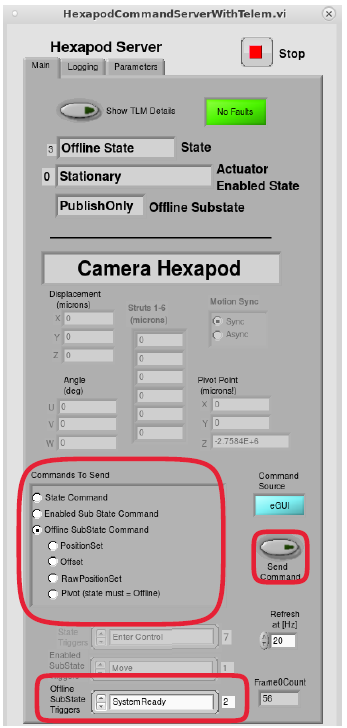
\includegraphics[width=1.79167in]{jira_imgs/1024.png}

\medskip }
\end{minipage}
\\ \cdashline{2-2}


 & Expected Result \\
 & \begin{minipage}[t]{15cm}{\footnotesize
The system transitions from the OfflineState/PublishOnly substate to the
OfflineState/AvailableState substate.\\[2\baselineskip]

\medskip }
\end{minipage} \\ \cdashline{2-2}

 & Actual Result \\
 & \begin{minipage}[t]{15cm}{\footnotesize
We transited the system to the OfflineState/AvailableState substate.

\medskip }
\end{minipage} \\ \cdashline{2-2}

 & Status: \textbf{ Initial Pass } \\ \hline

4 & Description \\
 & \begin{minipage}[t]{15cm}
{\footnotesize
\textbf{SWITCHING TO DDS MODE}\\
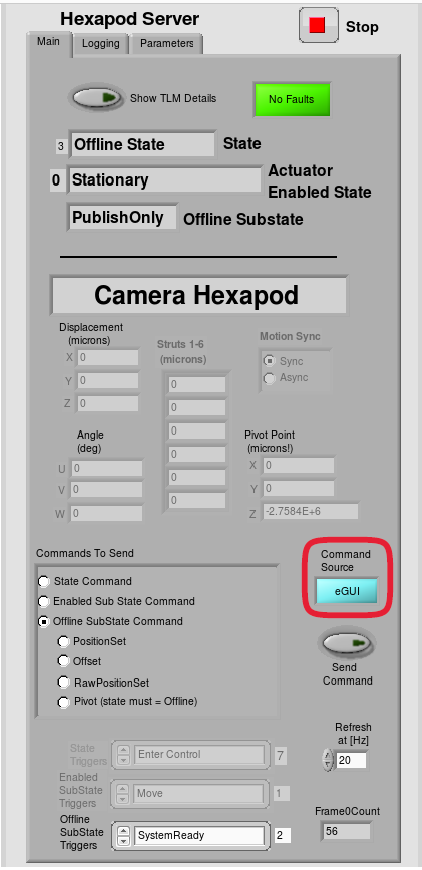
\includegraphics[width=1.68750in]{jira_imgs/1025.png}If the Command
Source does not show DDS, go to the Parameters tab, select DDS under the
Command Source and click the Set Cmd Source button.\\
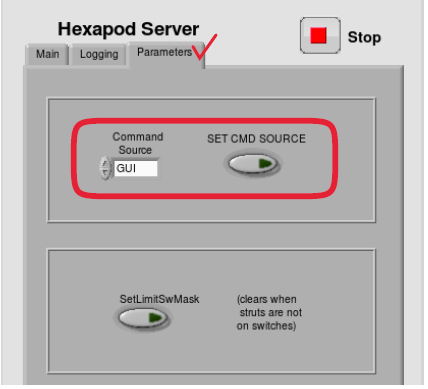
\includegraphics[width=2.34375in]{jira_imgs/1026.png}\textbf{Note:~If
the GUI is used after being set to DDS mode, the system will switch back
the Command Source to GUI and ignore any DDS commands. The Command
Source must show DDS in order to receive DDS commands.}

\medskip }
\end{minipage}
\\ \cdashline{2-2}


 & Expected Result \\
 & \begin{minipage}[t]{15cm}{\footnotesize
The system is capable of receiving/responding to DDS commands.

\medskip }
\end{minipage} \\ \cdashline{2-2}

 & Actual Result \\
 & \begin{minipage}[t]{15cm}{\footnotesize
We can do the DDS control.

\medskip }
\end{minipage} \\ \cdashline{2-2}

 & Status: \textbf{ Initial Pass } \\ \hline

5 & Description \\
 & \begin{minipage}[t]{15cm}
{\footnotesize
\textbf{OFFLINESTATE -\textgreater{} STANDBYSTATE}\\
The system receives an enterControl State Transition command through
DDS.

\medskip }
\end{minipage}
\\ \cdashline{2-2}


 & Expected Result \\
 & \begin{minipage}[t]{15cm}{\footnotesize
The system transitions into the StandbyState and is capable of
receiving/responding to DDS commands.

\medskip }
\end{minipage} \\ \cdashline{2-2}

 & Actual Result \\
 & \begin{minipage}[t]{15cm}{\footnotesize
We transited the system to the Standby state.

\medskip }
\end{minipage} \\ \cdashline{2-2}

 & Status: \textbf{ Initial Pass } \\ \hline

6 & Description \\
 & \begin{minipage}[t]{15cm}
{\footnotesize
\textbf{STANDBYSTATE -\textgreater{} DISABLEDSTATE}\\
From the StandbyState, send a start command through the DDS.

\medskip }
\end{minipage}
\\ \cdashline{2-2}


 & Expected Result \\
 & \begin{minipage}[t]{15cm}{\footnotesize
The system transitions into DisabledState after receiving/responding to
DDS command and the wrapper in the PXI real time controller looks for
the configuration file.\\[2\baselineskip]If the configuration file is
invalid or out of range, the system will transition into a Fault State

\medskip }
\end{minipage} \\ \cdashline{2-2}

 & Actual Result \\
 & \begin{minipage}[t]{15cm}{\footnotesize
We transited the system to the Disabled state.

\medskip }
\end{minipage} \\ \cdashline{2-2}

 & Status: \textbf{ Initial Pass } \\ \hline

7 & Description \\
 & \begin{minipage}[t]{15cm}
{\footnotesize
\textbf{DISABLEDSTATE -\textgreater{} ENABLEDSTATE}\\
From the DisabledState, send an enable state command through the DDS.\\
\textbf{}

\medskip }
\end{minipage}
\\ \cdashline{2-2}


 & Expected Result \\
 & \begin{minipage}[t]{15cm}{\footnotesize
The system transitions into the EnabledState/Stationary substate, the
motor drives are enabled, motor brakes are released and the system is
capable of receiving/responding to DDS commands.\\[2\baselineskip]

\medskip }
\end{minipage} \\ \cdashline{2-2}

 & Actual Result \\
 & \begin{minipage}[t]{15cm}{\footnotesize
We transited the system to the Enabled state.

\medskip }
\end{minipage} \\ \cdashline{2-2}

 & Status: \textbf{ Initial Pass } \\ \hline

8 & Description \\
 & \begin{minipage}[t]{15cm}
{\footnotesize
\textbf{FAULTSTATE}\\
If a Fault occurs in any of the other states, the system will
automatically transition to the Fault State. While in the Fault state,
send a clearError command through the DDS.\\
Note: If the fault that occurs goes through the interlock system, reset
the safety relay switch and send a clearError command.

\medskip }
\end{minipage}
\\ \cdashline{2-2}


 & Expected Result \\
 & \begin{minipage}[t]{15cm}{\footnotesize
The system transitions back to the OfflineState/PublishOnly substate and
is not capable of receiving/responding to DDS commands. (Go back to Step
3)

\medskip }
\end{minipage} \\ \cdashline{2-2}

 & Actual Result \\
 & \begin{minipage}[t]{15cm}{\footnotesize
Cleared error and transitioned back to OfflineState/Available

\medskip }
\end{minipage} \\ \cdashline{2-2}

 & Status: \textbf{ Initial Pass } \\ \hline

9 & Description \\
 & \begin{minipage}[t]{15cm}
{\footnotesize
\textbf{{MOVE TEST}}\\
\textbf{Section 3.1.2 of the attached Software Acceptance Test
Procedure\\
Test Sequence \#1 - Synchronous PositionSet and Move Commands}\\
In enabled/stationary state, send a positionSet command of (0um, 0um,
200um, 0 deg, 0 deg, 0 deg, s).

\medskip }
\end{minipage}
\\ \cdashline{2-2}


 & Expected Result \\
 & \begin{minipage}[t]{15cm}{\footnotesize
The hexapod does not move.

\medskip }
\end{minipage} \\ \cdashline{2-2}

 & Actual Result \\
 & \begin{minipage}[t]{15cm}{\footnotesize
Did not move.

\medskip }
\end{minipage} \\ \cdashline{2-2}

 & Status: \textbf{ Initial Pass } \\ \hline

10 & Description \\
 & \begin{minipage}[t]{15cm}
{\footnotesize
With the synchronous button enabled and in enabled/stationary state,
send a positionSet command of (2000um, -3500um, 200um, 0.01deg, -.05deg,
0.002deg).

\medskip }
\end{minipage}
\\ \cdashline{2-2}


 & Expected Result \\
 & \begin{minipage}[t]{15cm}{\footnotesize
The hexapod does not move

\medskip }
\end{minipage} \\ \cdashline{2-2}

 & Actual Result \\
 & \begin{minipage}[t]{15cm}{\footnotesize
Did not move.

\medskip }
\end{minipage} \\ \cdashline{2-2}

 & Status: \textbf{ Initial Pass } \\ \hline

11 & Description \\
 & \begin{minipage}[t]{15cm}
{\footnotesize
Send a move command.

\medskip }
\end{minipage}
\\ \cdashline{2-2}


 & Expected Result \\
 & \begin{minipage}[t]{15cm}{\footnotesize
\begin{itemize}
\tightlist
\item
  The hexapod moves to (2000um, -3500um, 200um, 0.01deg, -.05deg,
  0.002deg)
\item
  The actuators complete the move at nearly the same time.
\end{itemize}

\medskip }
\end{minipage} \\ \cdashline{2-2}

 & Actual Result \\
 & \begin{minipage}[t]{15cm}{\footnotesize
Moved to 1999,-3500,200,0.01,0.05,0.002)

\medskip }
\end{minipage} \\ \cdashline{2-2}

 & Status: \textbf{ Initial Pass } \\ \hline

12 & Description \\
 & \begin{minipage}[t]{15cm}
{\footnotesize
Record the corresponding DDS events that were generated.

\medskip }
\end{minipage}
\\ \cdashline{2-2}


 & Expected Result \\
 & \begin{minipage}[t]{15cm}{\footnotesize
\begin{itemize}
\tightlist
\item
  The controllerState.enabledSubstate goes to MOVING\_POINT\_TO\_POINT
  when the move begins and STATIONARY when the move ends.
\item
  An inPosition event is generated when the move is complete
\end{itemize}

\medskip }
\end{minipage} \\ \cdashline{2-2}

 & Actual Result \\
 & \begin{minipage}[t]{15cm}{\footnotesize
Deviation: Russell will need to modify the XML as the vendor's version
has no Boolean field for inPosition unlike for the Camera Rotator.

\medskip }
\end{minipage} \\ \cdashline{2-2}

 & Status: \textbf{ Pass w/ Deviation } \\ \hline

13 & Description \\
 & \begin{minipage}[t]{15cm}
{\footnotesize
\textbf{Section 3.1.2 of the attached Software Acceptance Test
Procedure\\
Test Sequence \#5 - Stop Commands}\\
In the enabled/stationary state, send a position set command of (0um,
0um, 5000um, 0deg, 0deg, 0deg)

\medskip }
\end{minipage}
\\ \cdashline{2-2}


 & Expected Result \\
 & \begin{minipage}[t]{15cm}{\footnotesize
The hexapod doesn't move.

\medskip }
\end{minipage} \\ \cdashline{2-2}

 & Actual Result \\
 & \begin{minipage}[t]{15cm}{\footnotesize
Does not move

\medskip }
\end{minipage} \\ \cdashline{2-2}

 & Status: \textbf{ Initial Pass } \\ \hline

14 & Description \\
 & \begin{minipage}[t]{15cm}
{\footnotesize
Send move command.

\medskip }
\end{minipage}
\\ \cdashline{2-2}


 & Expected Result \\
 & \begin{minipage}[t]{15cm}{\footnotesize
The hexapod begins to move.

\medskip }
\end{minipage} \\ \cdashline{2-2}

 & Actual Result \\
 & \begin{minipage}[t]{15cm}{\footnotesize
Begins to move.

\medskip }
\end{minipage} \\ \cdashline{2-2}

 & Status: \textbf{ Initial Pass } \\ \hline

15 & Description \\
 & \begin{minipage}[t]{15cm}
{\footnotesize
Before the hexapod completes its movement, send a stop command.

\medskip }
\end{minipage}
\\ \cdashline{2-2}


 & Expected Result \\
 & \begin{minipage}[t]{15cm}{\footnotesize
\begin{itemize}
\tightlist
\item
  The hexapod stops before reaching the previously commanded position
\end{itemize}

\medskip }
\end{minipage} \\ \cdashline{2-2}

 & Actual Result \\
 & \begin{minipage}[t]{15cm}{\footnotesize
Hexapod stopped

\medskip }
\end{minipage} \\ \cdashline{2-2}

 & Status: \textbf{ Initial Pass } \\ \hline

16 & Description \\
 & \begin{minipage}[t]{15cm}
{\footnotesize
Record the corresponding DDS events that were generated.

\medskip }
\end{minipage}
\\ \cdashline{2-2}


 & Expected Result \\
 & \begin{minipage}[t]{15cm}{\footnotesize
\begin{itemize}
\tightlist
\item
  The controllerState.enabledSubstate goes to CONTROLLED\_STOPPING when
  the stop is requested, then STATIONARY when the hexapod has halted.
\item
  No inPosition event is generated.
\end{itemize}

\medskip }
\end{minipage} \\ \cdashline{2-2}

 & Actual Result \\
 & \begin{minipage}[t]{15cm}{\footnotesize
It works.

\medskip }
\end{minipage} \\ \cdashline{2-2}

 & Status: \textbf{ Initial Pass } \\ \hline

17 & Description \\
 & \begin{minipage}[t]{15cm}
{\footnotesize
\textbf{Section 3.1.2 of the attached Software Acceptance Test
Procedure\\
Test Sequence \#9 - positionSet and moveLUT}\\
In enabled/stationary state, send a positionSet command of (0um, 0um,
200um, 0deg, 0deg, 0deg)

\medskip }
\end{minipage}
\\ \cdashline{2-2}


 & Expected Result \\
 & \begin{minipage}[t]{15cm}{\footnotesize
The hexapod doesn't move.

\medskip }
\end{minipage} \\ \cdashline{2-2}

 & Actual Result \\
 & \begin{minipage}[t]{15cm}{\footnotesize
Does not move

\medskip }
\end{minipage} \\ \cdashline{2-2}

 & Status: \textbf{ Initial Pass } \\ \hline

18 & Description \\
 & \begin{minipage}[t]{15cm}
{\footnotesize
In enabled/stationary state, send a positionSet command of (0um, 0um,
800um, 0deg, 0deg, 0deg)

\medskip }
\end{minipage}
\\ \cdashline{2-2}


 & Expected Result \\
 & \begin{minipage}[t]{15cm}{\footnotesize
The hexapod doesn't move.

\medskip }
\end{minipage} \\ \cdashline{2-2}

 & Actual Result \\
 & \begin{minipage}[t]{15cm}{\footnotesize
Does not move

\medskip }
\end{minipage} \\ \cdashline{2-2}

 & Status: \textbf{ Initial Pass } \\ \hline

19 & Description \\
 & \begin{minipage}[t]{15cm}
{\footnotesize
Send a moveLUT (180deg, 60deg, and 10deg) command

\medskip }
\end{minipage}
\\ \cdashline{2-2}


 & Expected Result \\
 & \begin{minipage}[t]{15cm}{\footnotesize
The hexapod moves to a different position than (0um, 0um, 800um, 0deg,
0deg, 0deg) and the actuators complete the move at nearly the same time.

\medskip }
\end{minipage} \\ \cdashline{2-2}

 & Actual Result \\
 & \begin{minipage}[t]{15cm}{\footnotesize
Hexapod moves to a different position(1699,199,920,0.03,-0.02,0.016)
(0,0,2970,0,0,0)

\medskip }
\end{minipage} \\ \cdashline{2-2}

 & Status: \textbf{ Initial Pass } \\ \hline

20 & Description \\
 & \begin{minipage}[t]{15cm}
{\footnotesize
{\textbf{OFFSET TEST}}\\
\textbf{Section 3.1.2 of the attached Software Acceptance Test
Procedure\\
Test Sequence \#4 - Synchronous Offset and Move Commands}\\
In enabled/stationary state, send a positionSet command of (500um,
800um, 200um, 0deg, 0deg, 0deg)

\medskip }
\end{minipage}
\\ \cdashline{2-2}

 & Test Data \\
 & \begin{minipage}[t]{15cm}{\footnotesize


\medskip }
\end{minipage} \\ \cdashline{2-2}

 & Expected Result \\
 & \begin{minipage}[t]{15cm}{\footnotesize
The hexapod doesn't move.

\medskip }
\end{minipage} \\ \cdashline{2-2}

 & Actual Result \\
 & \begin{minipage}[t]{15cm}{\footnotesize
Did not move.

\medskip }
\end{minipage} \\ \cdashline{2-2}

 & Status: \textbf{ Initial Pass } \\ \hline

21 & Description \\
 & \begin{minipage}[t]{15cm}
{\footnotesize
In enabled/stationary state, send an offset command of (0um, 0um,
2000um, 0deg, 0deg, 0deg).

\medskip }
\end{minipage}
\\ \cdashline{2-2}


 & Expected Result \\
 & \begin{minipage}[t]{15cm}{\footnotesize
The hexapod doesn't move.

\medskip }
\end{minipage} \\ \cdashline{2-2}

 & Actual Result \\
 & \begin{minipage}[t]{15cm}{\footnotesize

\medskip }
\end{minipage} \\ \cdashline{2-2}

 & Status: \textbf{ Initial Pass } \\ \hline

22 & Description \\
 & \begin{minipage}[t]{15cm}
{\footnotesize
Send a move command.~

\medskip }
\end{minipage}
\\ \cdashline{2-2}


 & Expected Result \\
 & \begin{minipage}[t]{15cm}{\footnotesize
\begin{itemize}
\tightlist
\item
  The hexapod moves only 2000um in Z from the previous position
\item
  The actuators complete the move at nearly the same time.
\end{itemize}

\medskip }
\end{minipage} \\ \cdashline{2-2}

 & Actual Result \\
 & \begin{minipage}[t]{15cm}{\footnotesize
Works.

\medskip }
\end{minipage} \\ \cdashline{2-2}

 & Status: \textbf{ Initial Pass } \\ \hline

23 & Description \\
 & \begin{minipage}[t]{15cm}
{\footnotesize
Record the corresponding DDS events that were generated.

\medskip }
\end{minipage}
\\ \cdashline{2-2}


 & Expected Result \\
 & \begin{minipage}[t]{15cm}{\footnotesize
\begin{itemize}
\tightlist
\item
  The controllerState.enabledSubstate goes to MOVING\_POINT\_TO\_POINT
  when the move begins and STATIONARY when the move ends
\item
  The inPosition event is True when the move finishes
\item
  The inPosition event is False when the enabledSubstate goes back to
  STATIONARY.
\end{itemize}

\medskip }
\end{minipage} \\ \cdashline{2-2}

 & Actual Result \\
 & \begin{minipage}[t]{15cm}{\footnotesize
Deviation: Russell will need to modify the XML as the vendor's version
has no Boolean field for inPosition unlike for the Camera Rotator.

\medskip }
\end{minipage} \\ \cdashline{2-2}

 & Status: \textbf{ Pass w/ Deviation } \\ \hline

24 & Description \\
 & \begin{minipage}[t]{15cm}
{\footnotesize
\textbf{Section 3.1.2 of the attached Software Acceptance Test
Procedure\\
Test Sequence \#2 -Pivot, PositionSet and Move Commands}\\
In enabled/stationary state, send a positionSet command of (2000um,
-3500um, 200um, 0.01deg, -0.05deg, 0.002deg)

\medskip }
\end{minipage}
\\ \cdashline{2-2}

 & Test Data \\
 & \begin{minipage}[t]{15cm}{\footnotesize
\textbf{Deviation:} Determine where the original pivot point is before
sending a pivot command of (0, 0, 0)

\medskip }
\end{minipage} \\ \cdashline{2-2}

 & Expected Result \\
 & \begin{minipage}[t]{15cm}{\footnotesize
The hexapod doesn't move.

\medskip }
\end{minipage} \\ \cdashline{2-2}

 & Actual Result \\
 & \begin{minipage}[t]{15cm}{\footnotesize
Original pivot is 0, 0, -2.7584E+6

\medskip }
\end{minipage} \\ \cdashline{2-2}

 & Status: \textbf{ Initial Pass } \\ \hline

25 & Description \\
 & \begin{minipage}[t]{15cm}
{\footnotesize
In the enabled/stationary state, send a pivot command of (0,0,0).

\medskip }
\end{minipage}
\\ \cdashline{2-2}


 & Expected Result \\
 & \begin{minipage}[t]{15cm}{\footnotesize
The actuator positions do not change but the hexapod position changes.

\medskip }
\end{minipage} \\ \cdashline{2-2}

 & Actual Result \\
 & \begin{minipage}[t]{15cm}{\footnotesize
Position data became -408, -3952, 199, 0.0100 -0.05 0.002

\medskip }
\end{minipage} \\ \cdashline{2-2}

 & Status: \textbf{ Initial Pass } \\ \hline

26 & Description \\
 & \begin{minipage}[t]{15cm}
{\footnotesize
In the enabled/stationary state, send a positionSet command of (2000um,
-3500um, 200um, 0.01deg, -0.05deg, 0.002deg)

\medskip }
\end{minipage}
\\ \cdashline{2-2}

 & Test Data \\
 & \begin{minipage}[t]{15cm}{\footnotesize
Deviation: Record any offset commands necessary to test before sending
the move command.\\
\textbf{{Note: Need input from Te-Wei on whether there are certain
offset commands to issue before sending the move command.}}

\medskip }
\end{minipage} \\ \cdashline{2-2}

 & Expected Result \\
 & \begin{minipage}[t]{15cm}{\footnotesize
The hexapod doesn't move.

\medskip }
\end{minipage} \\ \cdashline{2-2}

 & Actual Result \\
 & \begin{minipage}[t]{15cm}{\footnotesize
Does not move

\medskip }
\end{minipage} \\ \cdashline{2-2}

 & Status: \textbf{ Initial Pass } \\ \hline

27 & Description \\
 & \begin{minipage}[t]{15cm}
{\footnotesize
Send a move command.

\medskip }
\end{minipage}
\\ \cdashline{2-2}


 & Expected Result \\
 & \begin{minipage}[t]{15cm}{\footnotesize
Confirm the hexapod moves to the commanded position and the actuators
change position to account for the new pivot point.

\medskip }
\end{minipage} \\ \cdashline{2-2}

 & Actual Result \\
 & \begin{minipage}[t]{15cm}{\footnotesize
Moves to 2000, -3500, 200, 0.01, -0.05 0.002

\medskip }
\end{minipage} \\ \cdashline{2-2}

 & Status: \textbf{ Initial Pass } \\ \hline

28 & Description \\
 & \begin{minipage}[t]{15cm}
{\footnotesize
\textbf{{CONFIGURE LIMITS TEST}}\\
\textbf{Section 3.1.2 of the attached Software Acceptance Test
Procedure\\
Test Sequence \#6 - configureLimits Command}\\
In enabled/stationary state, send a configureLimits command of (12000um,
-1000um, 1000um, 0.1, -0.1, 0.05)

\medskip }
\end{minipage}
\\ \cdashline{2-2}


 & Expected Result \\
 & \begin{minipage}[t]{15cm}{\footnotesize
The command is rejected for being outside acceptable limits.

\medskip }
\end{minipage} \\ \cdashline{2-2}

 & Actual Result \\
 & \begin{minipage}[t]{15cm}{\footnotesize
Command rejected for x being outside limits

\medskip }
\end{minipage} \\ \cdashline{2-2}

 & Status: \textbf{ Initial Pass } \\ \hline

29 & Description \\
 & \begin{minipage}[t]{15cm}
{\footnotesize
In enabled/stationary state, send a configureLimits command of (1000um,
-1000um, 1000um, 0.1, -0.1, 0.05)

\medskip }
\end{minipage}
\\ \cdashline{2-2}


 & Expected Result \\
 & \begin{minipage}[t]{15cm}{\footnotesize
The command is accepted.

\medskip }
\end{minipage} \\ \cdashline{2-2}

 & Actual Result \\
 & \begin{minipage}[t]{15cm}{\footnotesize
Command Accepted

\medskip }
\end{minipage} \\ \cdashline{2-2}

 & Status: \textbf{ Initial Pass } \\ \hline

30 & Description \\
 & \begin{minipage}[t]{15cm}
{\footnotesize
In enabled/stationary state, send a positionSet command of (1200um, 0um,
200um, 0deg, 0deg, 0deg)

\medskip }
\end{minipage}
\\ \cdashline{2-2}


 & Expected Result \\
 & \begin{minipage}[t]{15cm}{\footnotesize
The command is rejected for being outside of range limits

\medskip }
\end{minipage} \\ \cdashline{2-2}

 & Actual Result \\
 & \begin{minipage}[t]{15cm}{\footnotesize
Command is accepted. Jira ticket filed~

\medskip }
\end{minipage} \\ \cdashline{2-2}

 & Issues found executing this step:  \\
 & \begin{minipage}[t]{13cm}{\footnotesize
\href{https://jira.lsstcorp.org/browse/DM-23092}{DM-23092}~~Check position limits for Hexapod move and offset commands

\medskip }
\end{minipage} \\ \cdashline{2-2}
 & Status: \textbf{ Fail } \\ \hline

31 & Description \\
 & \begin{minipage}[t]{15cm}
{\footnotesize
In enabled/stationary state, send a positionSet command of (990um,
990um, 200um, 0deg, 0deg, 0deg)

\medskip }
\end{minipage}
\\ \cdashline{2-2}


 & Expected Result \\
 & \begin{minipage}[t]{15cm}{\footnotesize
The command is rejected for being outside of range limits.

\medskip }
\end{minipage} \\ \cdashline{2-2}

 & Actual Result \\
 & \begin{minipage}[t]{15cm}{\footnotesize
Command is accepted.

\medskip }
\end{minipage} \\ \cdashline{2-2}

 & Issues found executing this step:  \\
 & \begin{minipage}[t]{13cm}{\footnotesize
\href{https://jira.lsstcorp.org/browse/DM-23092}{DM-23092}~~Check position limits for Hexapod move and offset commands

\medskip }
\end{minipage} \\ \cdashline{2-2}
 & Status: \textbf{ Fail } \\ \hline

32 & Description \\
 & \begin{minipage}[t]{15cm}
{\footnotesize
In enabled/stationary state, send a positionSet command of (500um,
500um, 200um, 0deg, 0.1 deg, 0.01deg)

\medskip }
\end{minipage}
\\ \cdashline{2-2}


 & Expected Result \\
 & \begin{minipage}[t]{15cm}{\footnotesize
The command is accepted.

\medskip }
\end{minipage} \\ \cdashline{2-2}

 & Actual Result \\
 & \begin{minipage}[t]{15cm}{\footnotesize
Command accepted.

\medskip }
\end{minipage} \\ \cdashline{2-2}

 & Status: \textbf{ Initial Pass } \\ \hline

33 & Description \\
 & \begin{minipage}[t]{15cm}
{\footnotesize
Send a move command.

\medskip }
\end{minipage}
\\ \cdashline{2-2}


 & Expected Result \\
 & \begin{minipage}[t]{15cm}{\footnotesize
The previously accepted command is executed.

\medskip }
\end{minipage} \\ \cdashline{2-2}

 & Actual Result \\
 & \begin{minipage}[t]{15cm}{\footnotesize
Move completed to correct position

\medskip }
\end{minipage} \\ \cdashline{2-2}

 & Status: \textbf{ Initial Pass } \\ \hline

34 & Description \\
 & \begin{minipage}[t]{15cm}
{\footnotesize
Record the DDS events that were generated.

\medskip }
\end{minipage}
\\ \cdashline{2-2}


 & Expected Result \\
 & \begin{minipage}[t]{15cm}{\footnotesize
The change is reflected in the settingsApplied event and the EUI.

\medskip }
\end{minipage} \\ \cdashline{2-2}

 & Actual Result \\
 & \begin{minipage}[t]{15cm}{\footnotesize
Change reflected in EUI, still checking EFD.

\medskip }
\end{minipage} \\ \cdashline{2-2}

 & Status: \textbf{ In Progress } \\ \hline

35 & Description \\
 & \begin{minipage}[t]{15cm}
{\footnotesize
{\textbf{CONFIGURE ACCELERATION TEST}}\\
\textbf{Section 3.1.2 of the attached Software Acceptance Test
Procedure\\
Test Sequence \#7 - configureAcceleration Command}\\
In enabled/stationary state, at a position of (0, 0, 0, 0, 0, 0) with
the velocity and acceleration values set to their nominal values, send a
positionSet command of (0um, 0um, 4900um, 0 deg, 0 deg, 0 deg, s).

\medskip }
\end{minipage}
\\ \cdashline{2-2}


 & Expected Result \\
 & \begin{minipage}[t]{15cm}{\footnotesize
The hexapod doesn't move.

\medskip }
\end{minipage} \\ \cdashline{2-2}

 & Actual Result \\
 & \begin{minipage}[t]{15cm}{\footnotesize
The Hexapod does not move

\medskip }
\end{minipage} \\ \cdashline{2-2}

 & Status: \textbf{ Initial Pass } \\ \hline

36 & Description \\
 & \begin{minipage}[t]{15cm}
{\footnotesize
Send a move command.

\medskip }
\end{minipage}
\\ \cdashline{2-2}


 & Expected Result \\
 & \begin{minipage}[t]{15cm}{\footnotesize
The move takes approximately 9 seconds to complete.

\medskip }
\end{minipage} \\ \cdashline{2-2}

 & Actual Result \\
 & \begin{minipage}[t]{15cm}{\footnotesize
Hexapod movement took approximately 9 seconds.~

\medskip }
\end{minipage} \\ \cdashline{2-2}

 & Status: \textbf{ Initial Pass } \\ \hline

37 & Description \\
 & \begin{minipage}[t]{15cm}
{\footnotesize
Send a configureAcceleration command of 1000.

\medskip }
\end{minipage}
\\ \cdashline{2-2}


 & Expected Result \\
 & \begin{minipage}[t]{15cm}{\footnotesize
~Confirm command is rejected for being outside of acceptable limits.

\medskip }
\end{minipage} \\ \cdashline{2-2}

 & Actual Result \\
 & \begin{minipage}[t]{15cm}{\footnotesize
Command rejected

\medskip }
\end{minipage} \\ \cdashline{2-2}

 & Status: \textbf{ Initial Pass } \\ \hline

38 & Description \\
 & \begin{minipage}[t]{15cm}
{\footnotesize
Send a configureAcceleration command of 100.

\medskip }
\end{minipage}
\\ \cdashline{2-2}


 & Expected Result \\
 & \begin{minipage}[t]{15cm}{\footnotesize
The command is accepted.~

\medskip }
\end{minipage} \\ \cdashline{2-2}

 & Actual Result \\
 & \begin{minipage}[t]{15cm}{\footnotesize
Command accepted

\medskip }
\end{minipage} \\ \cdashline{2-2}

 & Status: \textbf{ Initial Pass } \\ \hline

39 & Description \\
 & \begin{minipage}[t]{15cm}
{\footnotesize
In enabled/stationary state, send a postionSet command of (0um, 0um,
0um, 0 deg, 0 deg, 0 deg, s).

\medskip }
\end{minipage}
\\ \cdashline{2-2}


 & Expected Result \\
 & \begin{minipage}[t]{15cm}{\footnotesize
The hexapod doesn't move.

\medskip }
\end{minipage} \\ \cdashline{2-2}

 & Actual Result \\
 & \begin{minipage}[t]{15cm}{\footnotesize
Hexapod does not move

\medskip }
\end{minipage} \\ \cdashline{2-2}

 & Status: \textbf{ Initial Pass } \\ \hline

40 & Description \\
 & \begin{minipage}[t]{15cm}
{\footnotesize
Send a move command.~

\medskip }
\end{minipage}
\\ \cdashline{2-2}


 & Expected Result \\
 & \begin{minipage}[t]{15cm}{\footnotesize
It takes approximately 13 seconds to complete the commanded move with
the reduced acceleration value.

\medskip }
\end{minipage} \\ \cdashline{2-2}

 & Actual Result \\
 & \begin{minipage}[t]{15cm}{\footnotesize
Hexapod moved in approximately~ 13 seconds.

\medskip }
\end{minipage} \\ \cdashline{2-2}

 & Status: \textbf{ Initial Pass } \\ \hline

41 & Description \\
 & \begin{minipage}[t]{15cm}
{\footnotesize
Send a configureAcceleration command of 500 to return the acceleration
limit to its nominal value.

\medskip }
\end{minipage}
\\ \cdashline{2-2}


 & Expected Result \\
 & \begin{minipage}[t]{15cm}{\footnotesize
The command is accepted.

\medskip }
\end{minipage} \\ \cdashline{2-2}

 & Actual Result \\
 & \begin{minipage}[t]{15cm}{\footnotesize
Command accepted

\medskip }
\end{minipage} \\ \cdashline{2-2}

 & Status: \textbf{ Initial Pass } \\ \hline

42 & Description \\
 & \begin{minipage}[t]{15cm}
{\footnotesize
Record the corresponding DDS events that were generated.

\medskip }
\end{minipage}
\\ \cdashline{2-2}


 & Expected Result \\
 & \begin{minipage}[t]{15cm}{\footnotesize
The change is reflected in the settingsApplied event and the EUI.

\medskip }
\end{minipage} \\ \cdashline{2-2}

 & Actual Result \\
 & \begin{minipage}[t]{15cm}{\footnotesize
Changes were evident in EUI, still need to find EFD.

\medskip }
\end{minipage} \\ \cdashline{2-2}

 & Status: \textbf{ In Progress } \\ \hline

43 & Description \\
 & \begin{minipage}[t]{15cm}
{\footnotesize
\textbf{{CONFIGURE VELOCITY TEST}}\\
\textbf{Section 3.1.2 of the attached Software Acceptance Test
Procedure\\
Test Sequence \#8 - configureVelocity Command}\\
In enabled/stationary state, at a position of (0, 0, 0, 0, 0, 0), send a
configureVelocity command of (10000, .01, 100, .01).

\medskip }
\end{minipage}
\\ \cdashline{2-2}


 & Expected Result \\
 & \begin{minipage}[t]{15cm}{\footnotesize
This command is rejected for being outside of acceptable limits.

\medskip }
\end{minipage} \\ \cdashline{2-2}

 & Actual Result \\
 & \begin{minipage}[t]{15cm}{\footnotesize
Command rejected

\medskip }
\end{minipage} \\ \cdashline{2-2}

 & Status: \textbf{ Initial Pass } \\ \hline

44 & Description \\
 & \begin{minipage}[t]{15cm}
{\footnotesize
In enabled/stationary state, send a configureVelocity command of (100,
.01, 200, .01).~

\medskip }
\end{minipage}
\\ \cdashline{2-2}


 & Expected Result \\
 & \begin{minipage}[t]{15cm}{\footnotesize
This command is accepted.

\medskip }
\end{minipage} \\ \cdashline{2-2}

 & Actual Result \\
 & \begin{minipage}[t]{15cm}{\footnotesize
Command accepted

\medskip }
\end{minipage} \\ \cdashline{2-2}

 & Status: \textbf{ Initial Pass } \\ \hline

45 & Description \\
 & \begin{minipage}[t]{15cm}
{\footnotesize
In enabled/stationary state, send a positionSet command of (0, 0um,
2000um, 0 deg, 0 deg, 0 deg, s).

\medskip }
\end{minipage}
\\ \cdashline{2-2}


 & Expected Result \\
 & \begin{minipage}[t]{15cm}{\footnotesize
The command is accepted

\medskip }
\end{minipage} \\ \cdashline{2-2}

 & Actual Result \\
 & \begin{minipage}[t]{15cm}{\footnotesize
Command accepted

\medskip }
\end{minipage} \\ \cdashline{2-2}

 & Status: \textbf{ Initial Pass } \\ \hline

46 & Description \\
 & \begin{minipage}[t]{15cm}
{\footnotesize
Send a move command.~

\medskip }
\end{minipage}
\\ \cdashline{2-2}


 & Expected Result \\
 & \begin{minipage}[t]{15cm}{\footnotesize
It takes approximately 20 seconds to complete the commanded move.

\medskip }
\end{minipage} \\ \cdashline{2-2}

 & Actual Result \\
 & \begin{minipage}[t]{15cm}{\footnotesize
Approximately 20 seconds taken to move

\medskip }
\end{minipage} \\ \cdashline{2-2}

 & Status: \textbf{ Initial Pass } \\ \hline

47 & Description \\
 & \begin{minipage}[t]{15cm}
{\footnotesize
In enabled/stationary state, send a configureVelocity command of (100,
.01, 100, .01).~

\medskip }
\end{minipage}
\\ \cdashline{2-2}


 & Expected Result \\
 & \begin{minipage}[t]{15cm}{\footnotesize
This command is accepted.

\medskip }
\end{minipage} \\ \cdashline{2-2}

 & Actual Result \\
 & \begin{minipage}[t]{15cm}{\footnotesize
Accepted

\medskip }
\end{minipage} \\ \cdashline{2-2}

 & Status: \textbf{ Initial Pass } \\ \hline

48 & Description \\
 & \begin{minipage}[t]{15cm}
{\footnotesize
In enabled/stationary state, send an offset command of (0, 0um, 2000um,
0 deg, 0 deg, 0 deg).

\medskip }
\end{minipage}
\\ \cdashline{2-2}


 & Expected Result \\
 & \begin{minipage}[t]{15cm}{\footnotesize
This command is accepted

\medskip }
\end{minipage} \\ \cdashline{2-2}

 & Actual Result \\
 & \begin{minipage}[t]{15cm}{\footnotesize
Command accepted

\medskip }
\end{minipage} \\ \cdashline{2-2}

 & Status: \textbf{ Initial Pass } \\ \hline

49 & Description \\
 & \begin{minipage}[t]{15cm}
{\footnotesize
Send a move command.~

\medskip }
\end{minipage}
\\ \cdashline{2-2}


 & Expected Result \\
 & \begin{minipage}[t]{15cm}{\footnotesize
It takes approximately 40 seconds to complete the commanded move.

\medskip }
\end{minipage} \\ \cdashline{2-2}

 & Actual Result \\
 & \begin{minipage}[t]{15cm}{\footnotesize
Move completed in 40 seconds

\medskip }
\end{minipage} \\ \cdashline{2-2}

 & Status: \textbf{ Initial Pass } \\ \hline

50 & Description \\
 & \begin{minipage}[t]{15cm}
{\footnotesize
Record the corresponding DDS events that were generated:

\medskip }
\end{minipage}
\\ \cdashline{2-2}


 & Expected Result \\
 & \begin{minipage}[t]{15cm}{\footnotesize
The change is reflected in the settingsApplied event and the EUI.

\medskip }
\end{minipage} \\ \cdashline{2-2}

 & Actual Result \\
 & \begin{minipage}[t]{15cm}{\footnotesize
Changes reflected in EUI, still determining EFD

\medskip }
\end{minipage} \\ \cdashline{2-2}

 & Status: \textbf{ In Progress } \\ \hline

51 & Description \\
 & \begin{minipage}[t]{15cm}
{\footnotesize
\textbf{Section 3.3.2 of the attached Software Acceptance Test Procedure
Hexapod Action on State Commands}\\
In the Offline/PublishOnly state, send all commands

\medskip }
\end{minipage}
\\ \cdashline{2-2}


 & Expected Result \\
 & \begin{minipage}[t]{15cm}{\footnotesize
There is no change and command is rejected.

\medskip }
\end{minipage} \\ \cdashline{2-2}

 & Actual Result \\
 & \begin{minipage}[t]{15cm}{\footnotesize

\medskip }
\end{minipage} \\ \cdashline{2-2}

 & Status: \textbf{ Initial Pass } \\ \hline

52 & Description \\
 & \begin{minipage}[t]{15cm}
{\footnotesize
In the Offline/Available state, send an enterControl command

\medskip }
\end{minipage}
\\ \cdashline{2-2}


 & Expected Result \\
 & \begin{minipage}[t]{15cm}{\footnotesize
The system enters the Standby state.

\medskip }
\end{minipage} \\ \cdashline{2-2}

 & Actual Result \\
 & \begin{minipage}[t]{15cm}{\footnotesize
System enters standby state

\medskip }
\end{minipage} \\ \cdashline{2-2}

 & Status: \textbf{ Initial Pass } \\ \hline

53 & Description \\
 & \begin{minipage}[t]{15cm}
{\footnotesize
In the Standby state, send any command except start or exitControl

\medskip }
\end{minipage}
\\ \cdashline{2-2}


 & Expected Result \\
 & \begin{minipage}[t]{15cm}{\footnotesize
There is no change and command is rejected.

\medskip }
\end{minipage} \\ \cdashline{2-2}

 & Actual Result \\
 & \begin{minipage}[t]{15cm}{\footnotesize
Command rejected

\medskip }
\end{minipage} \\ \cdashline{2-2}

 & Status: \textbf{ Initial Pass } \\ \hline

54 & Description \\
 & \begin{minipage}[t]{15cm}
{\footnotesize
In the Standby state, send an exitControl command.

\medskip }
\end{minipage}
\\ \cdashline{2-2}


 & Expected Result \\
 & \begin{minipage}[t]{15cm}{\footnotesize
The system transitions into the Offline/Available state.

\medskip }
\end{minipage} \\ \cdashline{2-2}

 & Actual Result \\
 & \begin{minipage}[t]{15cm}{\footnotesize
Transitions to Offline/Available

\medskip }
\end{minipage} \\ \cdashline{2-2}

 & Status: \textbf{ Initial Pass } \\ \hline

55 & Description \\
 & \begin{minipage}[t]{15cm}
{\footnotesize
In the Standby state, send a start command.

\medskip }
\end{minipage}
\\ \cdashline{2-2}


 & Expected Result \\
 & \begin{minipage}[t]{15cm}{\footnotesize
The system transitions into the Disabled state.

\medskip }
\end{minipage} \\ \cdashline{2-2}

 & Actual Result \\
 & \begin{minipage}[t]{15cm}{\footnotesize
Transitions to disabled state

\medskip }
\end{minipage} \\ \cdashline{2-2}

 & Status: \textbf{ Initial Pass } \\ \hline

56 & Description \\
 & \begin{minipage}[t]{15cm}
{\footnotesize
In the Disabled state, send any command except for the enabled or
standby command.

\medskip }
\end{minipage}
\\ \cdashline{2-2}


 & Expected Result \\
 & \begin{minipage}[t]{15cm}{\footnotesize
There is no change and the command is rejected.

\medskip }
\end{minipage} \\ \cdashline{2-2}

 & Actual Result \\
 & \begin{minipage}[t]{15cm}{\footnotesize
Command rejected

\medskip }
\end{minipage} \\ \cdashline{2-2}

 & Status: \textbf{ Initial Pass } \\ \hline

57 & Description \\
 & \begin{minipage}[t]{15cm}
{\footnotesize
In the Disabled state, send the standby command.

\medskip }
\end{minipage}
\\ \cdashline{2-2}


 & Expected Result \\
 & \begin{minipage}[t]{15cm}{\footnotesize
The system transitions into the Standby state.

\medskip }
\end{minipage} \\ \cdashline{2-2}

 & Actual Result \\
 & \begin{minipage}[t]{15cm}{\footnotesize
Transitions to standby state

\medskip }
\end{minipage} \\ \cdashline{2-2}

 & Status: \textbf{ Initial Pass } \\ \hline

58 & Description \\
 & \begin{minipage}[t]{15cm}
{\footnotesize
In the Disabled state, send the enable command.

\medskip }
\end{minipage}
\\ \cdashline{2-2}


 & Expected Result \\
 & \begin{minipage}[t]{15cm}{\footnotesize
The system transitions into the Enabled/Stationary state.

\medskip }
\end{minipage} \\ \cdashline{2-2}

 & Actual Result \\
 & \begin{minipage}[t]{15cm}{\footnotesize
Transitions to enabled state

\medskip }
\end{minipage} \\ \cdashline{2-2}

 & Status: \textbf{ Initial Pass } \\ \hline

59 & Description \\
 & \begin{minipage}[t]{15cm}
{\footnotesize
In the Enabled/Stationary state, send either the enterControl command,
exitControl command, start command, clearError command, or enable
command.

\medskip }
\end{minipage}
\\ \cdashline{2-2}


 & Expected Result \\
 & \begin{minipage}[t]{15cm}{\footnotesize
There is no change and command is rejected.

\medskip }
\end{minipage} \\ \cdashline{2-2}

 & Actual Result \\
 & \begin{minipage}[t]{15cm}{\footnotesize
Command rejected

\medskip }
\end{minipage} \\ \cdashline{2-2}

 & Status: \textbf{ Initial Pass } \\ \hline

60 & Description \\
 & \begin{minipage}[t]{15cm}
{\footnotesize
In the Enabled/Stationary state, send a disable command.

\medskip }
\end{minipage}
\\ \cdashline{2-2}


 & Expected Result \\
 & \begin{minipage}[t]{15cm}{\footnotesize
The system transitions into Disabled state.

\medskip }
\end{minipage} \\ \cdashline{2-2}

 & Actual Result \\
 & \begin{minipage}[t]{15cm}{\footnotesize
Transitioned to disabled state

\medskip }
\end{minipage} \\ \cdashline{2-2}

 & Status: \textbf{ Initial Pass } \\ \hline

61 & Description \\
 & \begin{minipage}[t]{15cm}
{\footnotesize
In the Fault state, send any command except the clearError command.

\medskip }
\end{minipage}
\\ \cdashline{2-2}


 & Expected Result \\
 & \begin{minipage}[t]{15cm}{\footnotesize
There is no change and command is rejected.

\medskip }
\end{minipage} \\ \cdashline{2-2}

 & Actual Result \\
 & \begin{minipage}[t]{15cm}{\footnotesize

\medskip }
\end{minipage} \\ \cdashline{2-2}

 & Status: \textbf{ Initial Pass } \\ \hline

62 & Description \\
 & \begin{minipage}[t]{15cm}
{\footnotesize
In the Fault state, send the clearError command.

\medskip }
\end{minipage}
\\ \cdashline{2-2}


 & Expected Result \\
 & \begin{minipage}[t]{15cm}{\footnotesize
The system transitions into the Offline/PublishOnly state.

\medskip }
\end{minipage} \\ \cdashline{2-2}

 & Actual Result \\
 & \begin{minipage}[t]{15cm}{\footnotesize

\medskip }
\end{minipage} \\ \cdashline{2-2}

 & Status: \textbf{ Initial Pass } \\ \hline

63 & Description \\
 & \begin{minipage}[t]{15cm}
{\footnotesize
\textbf{Section 4 of the attached Software Acceptance Test Procedure}\\
In the Enabled/Stationary state, unplug a motor encoder cable for one of
the actuators.\textbf{}\\

\medskip }
\end{minipage}
\\ \cdashline{2-2}


 & Expected Result \\
 & \begin{minipage}[t]{15cm}{\footnotesize
A Drive Fault error event is created and the system transitions to Fault
state.

\medskip }
\end{minipage} \\ \cdashline{2-2}

 & Actual Result \\
 & \begin{minipage}[t]{15cm}{\footnotesize

\medskip }
\end{minipage} \\ \cdashline{2-2}

 & Status: \textbf{ Not Executed } \\ \hline

64 & Description \\
 & \begin{minipage}[t]{15cm}
{\footnotesize
In the Enabled/Stationary state, unplug a linear encoder cable for one
of the actuators.

\medskip }
\end{minipage}
\\ \cdashline{2-2}


 & Expected Result \\
 & \begin{minipage}[t]{15cm}{\footnotesize
A Drive Fault error event is created and the system transitions to Fault
state.

\medskip }
\end{minipage} \\ \cdashline{2-2}

 & Actual Result \\
 & \begin{minipage}[t]{15cm}{\footnotesize

\medskip }
\end{minipage} \\ \cdashline{2-2}

 & Status: \textbf{ Not Executed } \\ \hline

65 & Description \\
 & \begin{minipage}[t]{15cm}
{\footnotesize
Unplug a motor power cable from one of the actuators and command a
PositionSet/Move.

\medskip }
\end{minipage}
\\ \cdashline{2-2}


 & Expected Result \\
 & \begin{minipage}[t]{15cm}{\footnotesize
A Following Error event is created and the system transitions to Fault
state.

\medskip }
\end{minipage} \\ \cdashline{2-2}

 & Actual Result \\
 & \begin{minipage}[t]{15cm}{\footnotesize

\medskip }
\end{minipage} \\ \cdashline{2-2}

 & Status: \textbf{ Not Executed } \\ \hline

66 & Description \\
 & \begin{minipage}[t]{15cm}
{\footnotesize
Activate an extension limit switch on one of the actuators by removing
the limit switch cover and manually tripping.

\medskip }
\end{minipage}
\\ \cdashline{2-2}


 & Expected Result \\
 & \begin{minipage}[t]{15cm}{\footnotesize
An Extended Limit Switch error event is created and the system
transitions into Fault state.

\medskip }
\end{minipage} \\ \cdashline{2-2}

 & Actual Result \\
 & \begin{minipage}[t]{15cm}{\footnotesize

\medskip }
\end{minipage} \\ \cdashline{2-2}

 & Status: \textbf{ Not Executed } \\ \hline

67 & Description \\
 & \begin{minipage}[t]{15cm}
{\footnotesize
Activate a retraction limit switch on one of the actuators by removing
the limit switch cover and manually tripping.

\medskip }
\end{minipage}
\\ \cdashline{2-2}


 & Expected Result \\
 & \begin{minipage}[t]{15cm}{\footnotesize
A Retracted Limit Switch error event is created and the system
transitions into Fault state.

\medskip }
\end{minipage} \\ \cdashline{2-2}

 & Actual Result \\
 & \begin{minipage}[t]{15cm}{\footnotesize

\medskip }
\end{minipage} \\ \cdashline{2-2}

 & Status: \textbf{ Not Executed } \\ \hline

68 & Description \\
 & \begin{minipage}[t]{15cm}
{\footnotesize
Unplug the Ethercat cable between the control PC and the first Copley
XE2 drive.

\medskip }
\end{minipage}
\\ \cdashline{2-2}


 & Expected Result \\
 & \begin{minipage}[t]{15cm}{\footnotesize
An Ethercat Lost event is created and the system transitions to Fault
state.

\medskip }
\end{minipage} \\ \cdashline{2-2}

 & Actual Result \\
 & \begin{minipage}[t]{15cm}{\footnotesize

\medskip }
\end{minipage} \\ \cdashline{2-2}

 & Status: \textbf{ Not Executed } \\ \hline

\end{longtable}


\newpage
\appendix
%Make sure lsst-texmf/bin/generateAcronyms.py is in your path
\section{Acronyms used in this document}\label{sec:acronyms}
\addtocounter{table}{-1}
\begin{longtable}{p{0.145\textwidth}p{0.8\textwidth}}\hline
\textbf{Acronym} & \textbf{Description}  \\\hline

EFD & Engineering and Facility Database \\\hline
GUI & Graphical User Interface \\\hline
LSST & Large Synoptic Survey Telescope \\\hline
LUT & Look-Up Table \\\hline
PMCS & Project Management Controls System \\\hline
Source & A single detection of an astrophysical object in an image, the characteristics for which are stored in the Source Catalog of the DRP database. The association of Sources that are non-moving lead to Objects; the association of moving Sources leads to Solar System Objects. (Note that in non-LSST usage "source" is often used for what LSST calls an Object.) \\\hline
\end{longtable}


\end{document}
